%\subsection{acceptance}
%\subsection{efficiency: peak counting}
%\subsection{efficiency: hit-by-hit}
%\subsection{Tag-and-probe technique}
\chapter{Efficiency}

We explore the data-driven tag and probe (T\&P) method to estimate single-muon trigger, identification, and tracking efficiencies. 
A comparison of the results obtained by applying the technique to both data and MC simulation allows to estimate related systematic uncertainties. 

The procedure is identical to that used in the previous analysis iteration, based in the 2010 \PbPb dataset, documented in Ref.~\cite{CMS_AN_2011_062}. 
The T\&P analysis is done using the official tag and probe framework, % tbd REF
as employed for example in Ref.~\cite{CMS_AN_2011_062, CMS_AN_2010-140}. 
The \Jpsi signal resonance is used to differentiate signal from background. 
Two tag-probe invariant mass distributions are formed, in the vicinity of the \Jpsi nominal mass, according to whether the probe passes or fails the criteria for which the efficiency is being measured.  
The two mass distributions are then fit simultaneously, and the efficiency $\varepsilon$ (and its uncertainty) is extracted as a common parameter in the fit, 
%
\begin{linenomath}
\begin{align}
  N_{\text{pass}} &= \varepsilon \times N_{\text{probes}} \,,\\
  N_{\text{fail}} &= (1 - \varepsilon ) \times N_{\text{probes}} \,,\nonumber
\end{align}
\end{linenomath}
%
where $N_{\text{probes}}$, $N_{\text{pass}}$, and $N_{\text{fail}}$
are the number of all probes, passing probes, and failing probes, respectively. 

Some challenges arise in measuring the tracking efficiency because in heavy ions fake and
tracking efficiency can be ``correlated'' due to the high
multiplicity, \ie one can have a fake match in events in which one has
removed the true match. 
%This problem was first encountered in the \Z
%analysis. 
Yet another problem is that measuring
the matching efficiency %($\varepsilon_{\text{M}}$) 
between a standalone muon and an inner track (necessary to promote a standalone
muon to a global muon) is not straightforward in heavy ions~\cite{CMS_AN_2011_062}. 
Furthermore, to fit failing tag and probe pairs becomes challenging due to the poor
resolution of the standalone (STA) muons.
%
%To measure the standalone muon to inner track matching
%efficiency, one could try to use as probes standalone muons and
%define passing probes as probes that are also global muons. 
%%
%But then one can get failing probes due to the following reasons:
%\begin{enumerate}
%\item The probe was a true muon with an outer track and an inner track
%  but failed the global matching criteria (that is a loss due to the
%  true matching efficiency which you want to measure)
%\item The probe was a true muon but the
%  inner track was a fake match. This could happen due to the very high inner tracker occupancy combined with tracking inefficiency. Then one would expect in most cases this
%  probe not to be a global muon, due to the tighter matching criteria.
%\item The probe was a fake muon, but the inner track part was a true muon. This is probably highly unlikely due to
%  the lower occupancy in the muon chambers, but possible.
%\item The probe was a fake muon, as well as the
%  inner track part. It could still survive the global muon criteria,
%  but independent of that, it is not a muon from the resonance decay
%  that is used for the Tag and Probe.
%\end{enumerate}
%
%If one uses the standalone momentum measurement, cases 1. and 2. will
%end up in the \Jpsi peak of the failing probe distribution, while 3. and 4. would just
%contribute to the background continuum. But case 2. is not failing
%because of the matching efficiency, but because of the tracking
%efficiency. So in this case, one would not measure $(1 -
%\varepsilon_{\text{M}})$ with the failing probes.
%
%If, however one uses the inner track momentum measurement, case
%2. would not end up in the peak of the failing probe distribution, as
%the track was a fake track. Instead, now case 3. would end up in the
%peak of the failing probes. Again, one would not measure directly $(1
%- \varepsilon_{\text{M}})$ with the failing probes, even though it might be
%much closer to the correct value, as case 3. is much less likely than
%case 2..
%
%One could completely ignore the failing probes and only fit the
%passing probes, but then one is left with the problem of not knowing
%the uncertainty on the efficiency: one cannot use binomial statistics
%due to the background.
%
In general, %instead, 
we will compare the efficiency estimations found with T\&P in Monte Carlo simulation and  data as a cross check of the Monte Carlo based efficiency corrections. 

Tags are selected as high quality, global muons, which are matched to the single muon trigger path HLT\_HIL1SingleMu0\_HighQ,  
%Tags are selected as muons which are matched to either the HLT\_HIL1DoubleMu0\_HighQ or the HLT\_HIL2DoubleMu3 trigger (our two triggers with the lowest \pt thresholds)
that also pass the offline muon selection used in the data analysis.
% and that are within the single muon acceptance.
%
These tag muons are combined with probe muons to form tag-probe
pairs. The probe muon selection depends on the efficiency being measured.
A condition is applied to the probes which are split into the passing and failing probe categories. 
It is the efficiency of this condition relative to all probes that is measured with T\&P.
%
We have used the following three probe categories to measure the inner-track reconstruction,
muon reconstruction and identification, and muon trigger efficiencies:
%
\begin{itemize}
\item inner-track reconstruction efficiency (including inner to
  outer track matching, and track quality criteria): %and the quality cuts as those are inner track selections:
  \begin{itemize}
  \item probe: a standalone muon (the four-momentum information is taken from the
    standalone part exclusively)
  \item passing probe: probe that is also a global muon passing the quality cuts
  \end{itemize}
\item global muon reconstruction and identification efficiency (relative to tracker muon)
%(including the  inner to outer track matching efficiency):
  \begin{itemize}
  \item probe: tracker muon %inner track of type \verb=hiSelectedTrack=   whithin the acceptance
  \item passing probe: probe that can be matched to a global muon and that fulfills the analysis muon selection criteria
  \end{itemize}
\item trigger efficiency:
  \begin{itemize}
  \item probe: (global) muon that satisfies the offline analysis selection criteria
%global muon that fulfills all quality cuts in the acceptance
    \item passing probe: probe that can be matched to (one leg of) HLT\_HIL1DoubleMu0\_HighQ trigger path.
  \end{itemize}
\end{itemize}

In order to attempt a reduction of the background level, further selection criteria have been tried. 
%For example, when evaluating efficiencies other than trigger, matching HLT\_HIL1DoubleMu0\_HighQ is applied.
A requirement on the dimuon $\pt > 6.5 \GeVc$ is applied and as well as a single muon  $\pt > 4.0 \GeVc$
In all cases, identical selection criteria are applied to both data and simulation: this is necessary for yielding reliable systematic estimates based on data-MC efficiency results comparison. 

The efficiency in simulation is measured using T\&P on a prompt \Jpsi sample.  
The MC sample is weighted for the centrality dependence (which scales with \ncoll) and for the relative weights between the different \pt bins used in the sample production. 
% as listed in \tab{tab:wfilter}. 
While the T\&P framework allows for weighted samples, the uncertainty estimates using the current version of RooFit for weighted datasets is not accurate. 
%properly taking into account the weighted errors when calculating the error on the fit result. 
However, employing large MC statistics, we will take the size of the corresponding errors to be negligible. 
%Therefore the error bars on the MC Tag and Probe efficiencies are not plotted. However, as we have a lot of MC statistics, we could estimate the size of the errors to be negligible. Figure~\ref{fig:tnpTrkErr} illustrate the small size of the error for one \pt bin of the \Jpsi simulation in 6-9GeV/c in bin of \Jpsi \pt, not weighted. It is 2\% of 84\% for that bin.

The estimation of the systematic uncertainty will be assigned by comparing results between data and simulation.  
%Currently, only the results extracted from data are provided; the T\&P MC results are still being finalized.  
%Systematic uncertainty can be estimated once we get the efficiencies in MC.
%
We also note that only results above the single-muon \pt of 4.0\GeVc are within the acceptance used in the analysis. 
This tends to reach the muon efficiency plateau, and is less affected by systematics related to the detailed description of the efficiency turn-on. 


%TBD: describe the fit model!!!!!

\subsubsection{Trigger efficiency}

The trigger efficiency is, in general, the easiest one to fit for, given the cleaner probe sample. The signal shape is describe by a Crystal Ball plus a Gaussian. The addition of the Gaussian is motivated to describe varying detector resolution. The parameters in the Crystal Ball as well as the width of the Gaussian are free parameters of the fit. The background is described by an exponential function. 
%In the MC case, we proceed similarly using a Crystal Ball plus a Gaussian for the signal and an exponential background.  

Figure~\ref{fig:tnpTrigFit} shows fits to the passing and failing samples of T\&P pairs for the
trigger efficiency measurement, using the integrated data and MC samples. % in data, respectively. 
%TBD: add MB integrated fits in data and MC
%
%The \pt and $\eta$ dependence of the trigger efficiency  compares rather well between 2011 and 2010 and is shown in  \fig{fig:tnpTrigEff} left column for \Jpsi \pt$> 6.5$~Gev/c. 
%
%The \pt and $\eta$ integrated trigger  efficiency is $92.6\pm0.6$\%  for the HLT\_HIL1DoubleMu0\_HighQ % and $78.4\pm0.7$\%  forHLT\_HIL2DoubleMu3 
%in the 2011 data. 
Figure~\ref{fig:tnpTrigEff} shows the trigger efficiency measured as a function of probe \pt and pseudo-rapidity.
Also shown is the trigger efficiency as function of centrality which, as expected, shows no significant dependence. 
A reasonable agreement between data and simulation is obtained especially in the most peripheral bins. 


\begin{figure}[hp]
  \begin{center}
    \subfigure[Data]{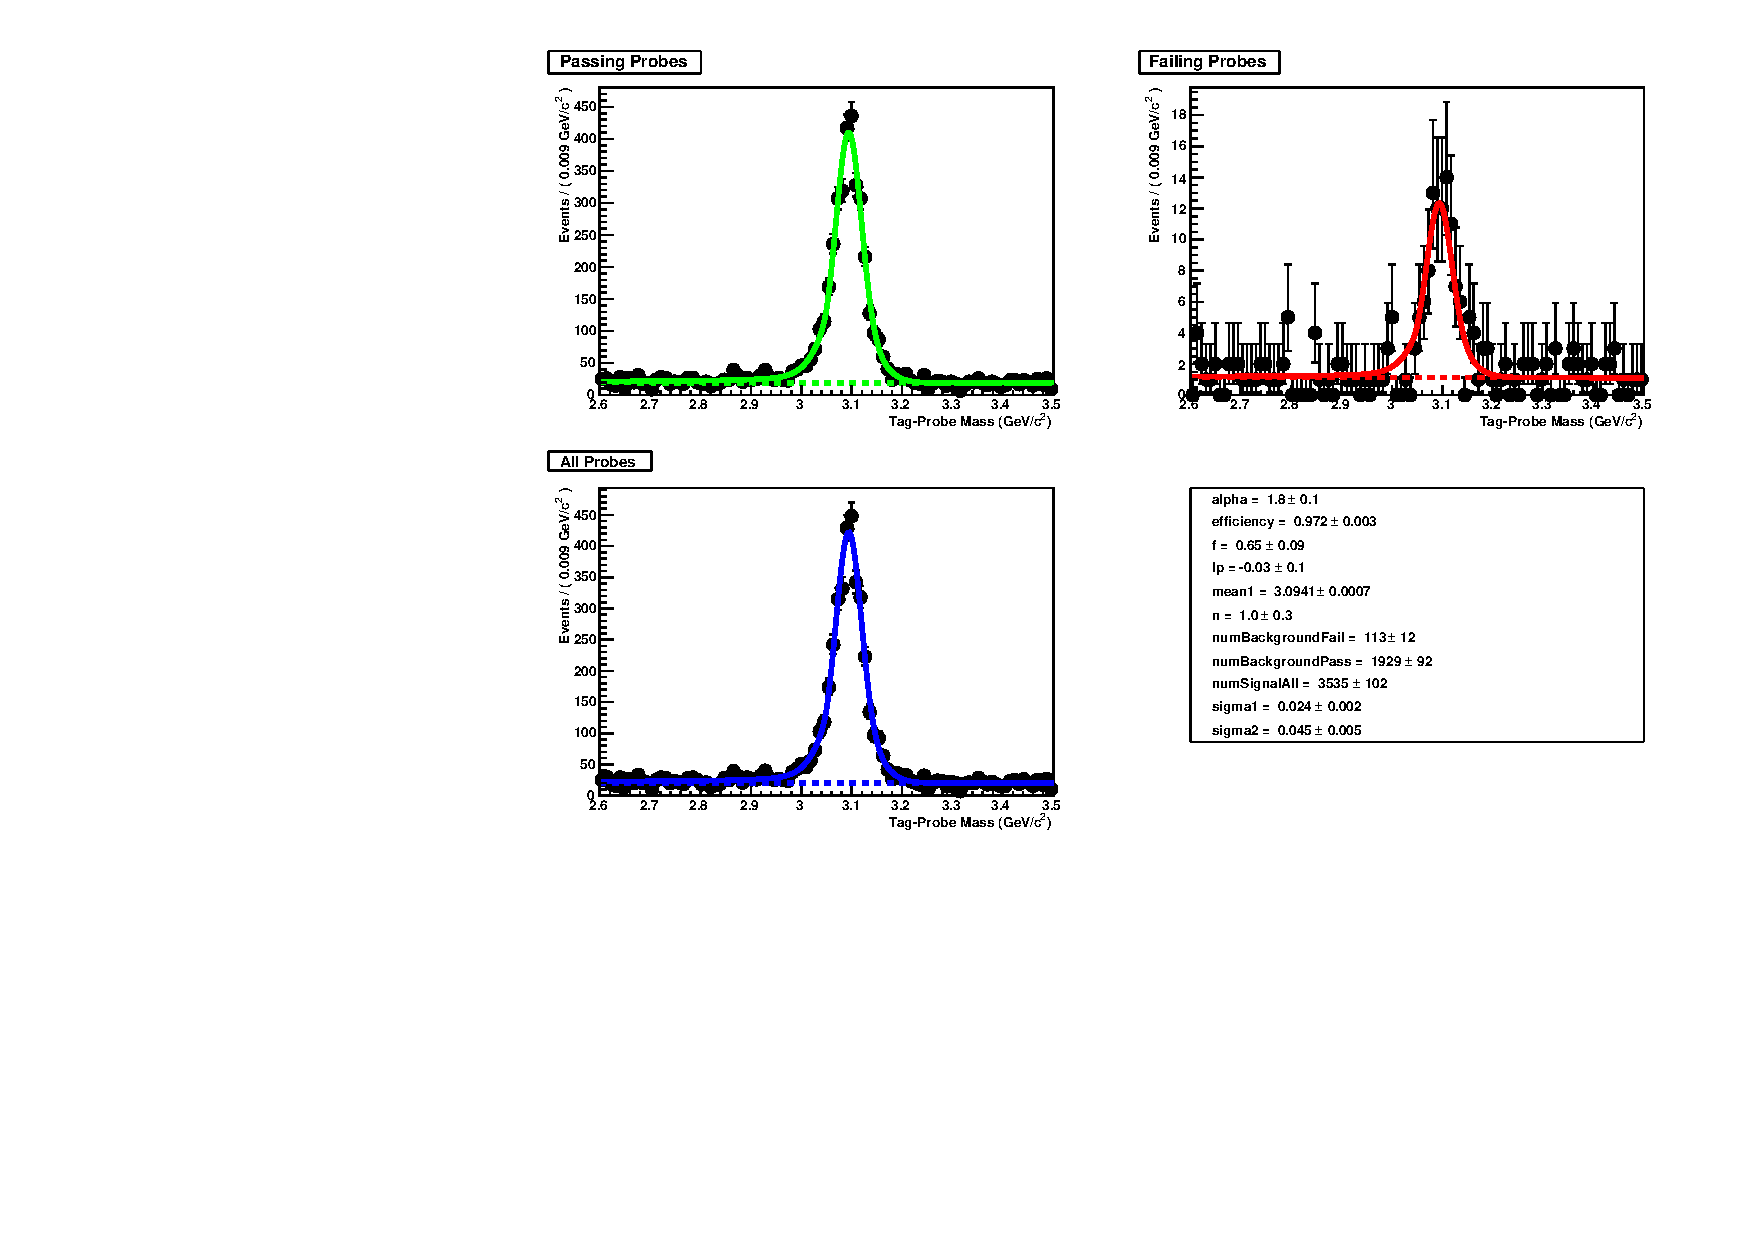
\includegraphics[width=0.9\textwidth]{figures/efficiency/RD_Trg_massfit_0100_HLTL1}}\hspace{1em}
    \subfigure[Monte Carlo]{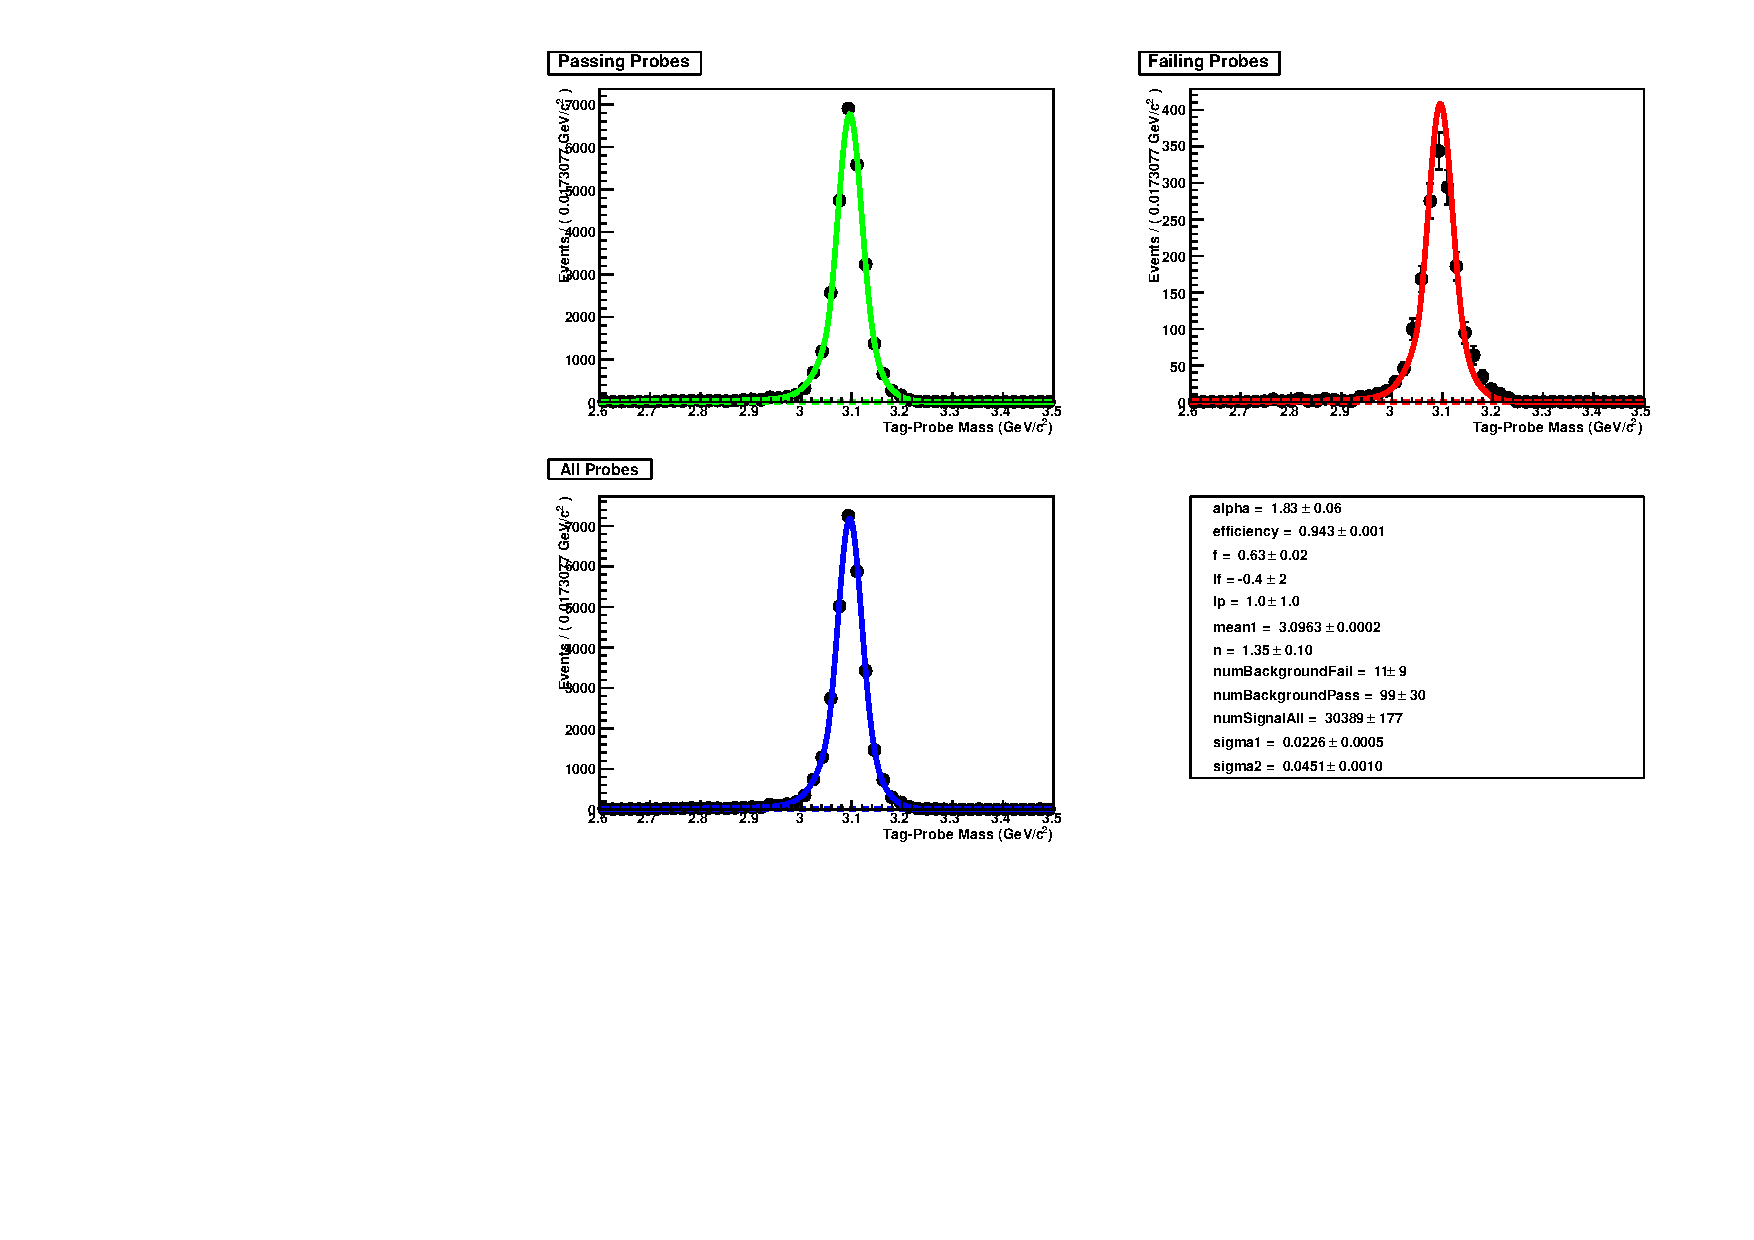
\includegraphics[width=0.9\textwidth]{figures/efficiency/MC_Trg_massfit_0100_HLTL1}}
    \caption{Examples of tag-probe pair mass fits used to extract the trigger efficiency for data and MC.}%TBD add MB inetagretyd plot in data and MC!
    \label{fig:tnpTrigFit}
  \end{center}
\end{figure}


\begin{figure}[hp]
  \begin{center}
    \subfigure[Trigger efficiency dependence on muon $\pt$.]{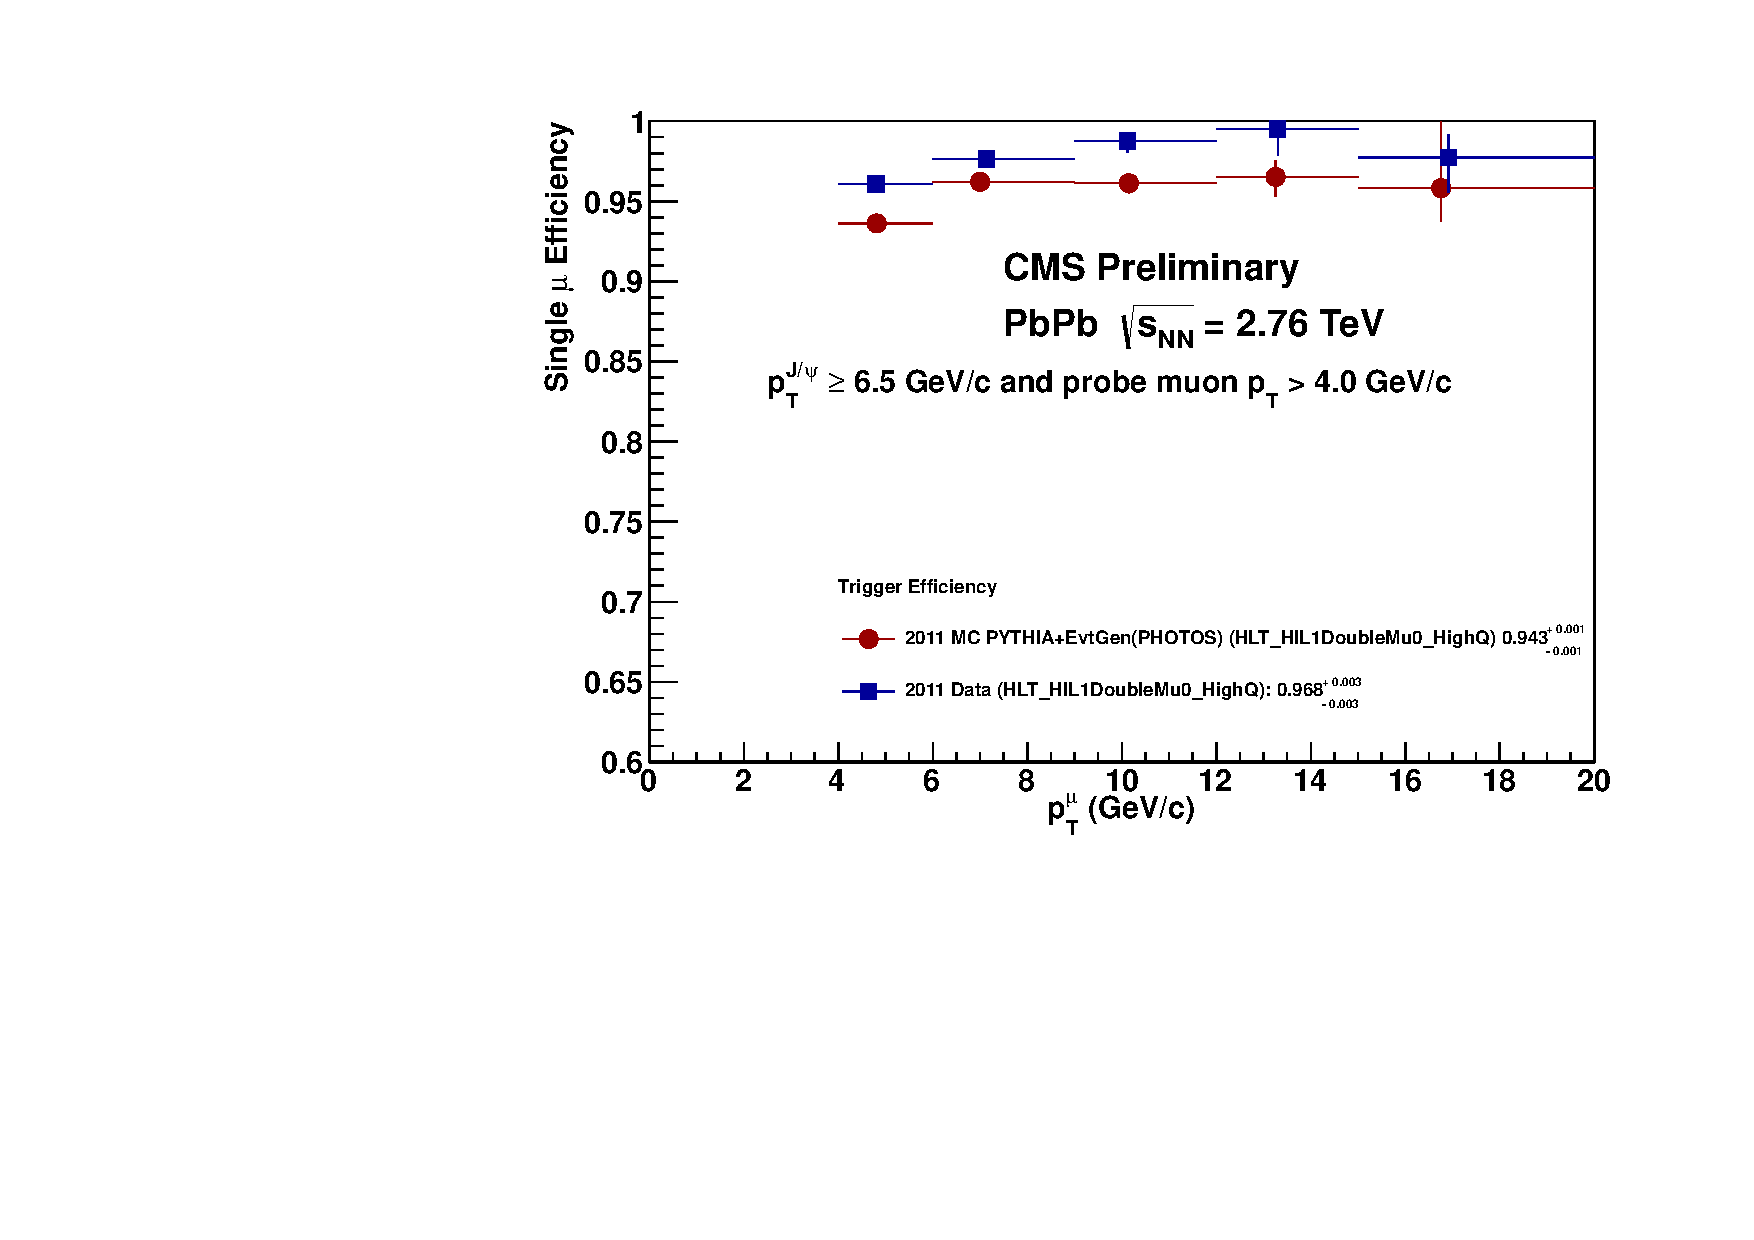
\includegraphics[width=0.6\textwidth]{figures/efficiency/Trg_Comp_HI_pt_RD_MC_HighPt_notriggermatched}}  \\ %\hspace{1em}
    \subfigure[Trigger efficiency dependence on muon $\eta$.]{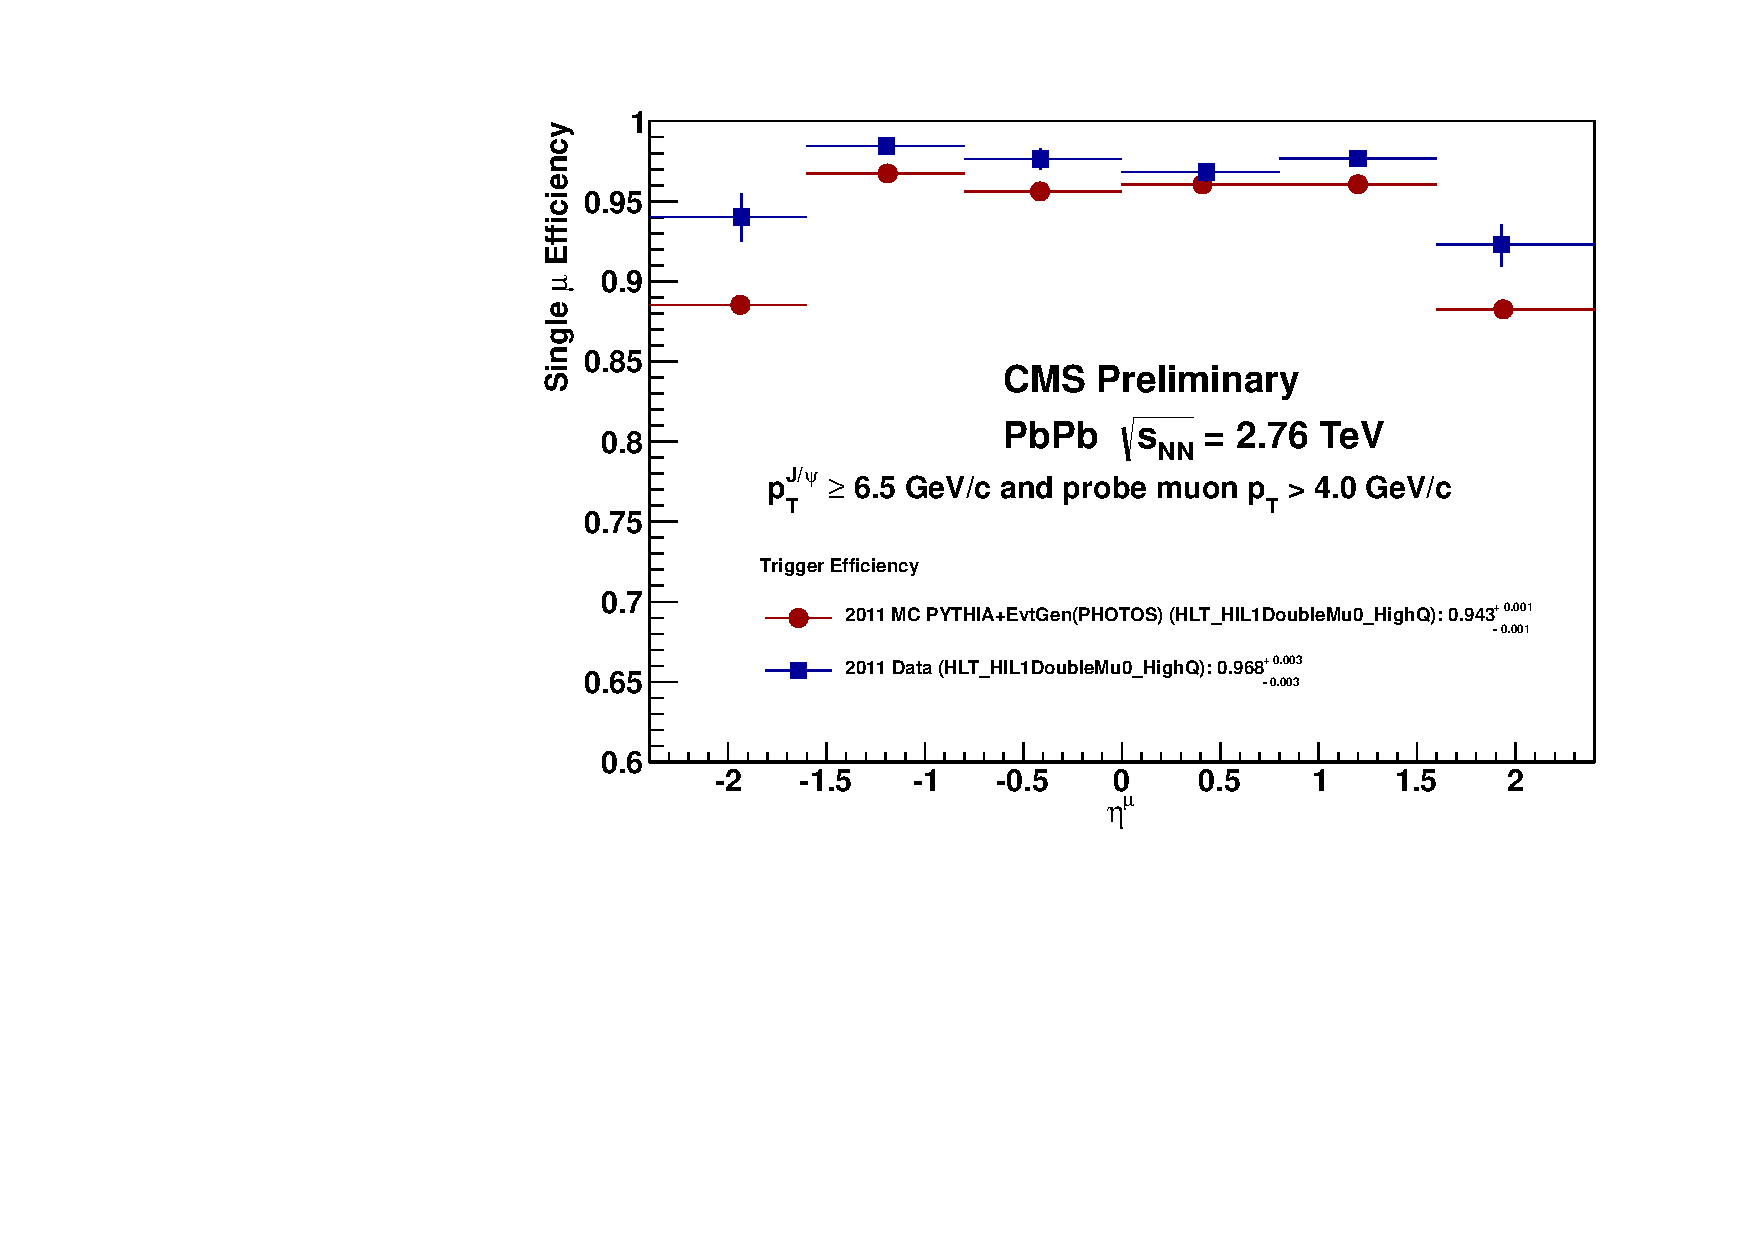
\includegraphics[width=0.6\textwidth]{figures/efficiency/Trg_Comp_HI_eta_RD_MC_HighPt_notriggermatched}} \\
    \subfigure[Trigger efficiency dependence on event centrality.]{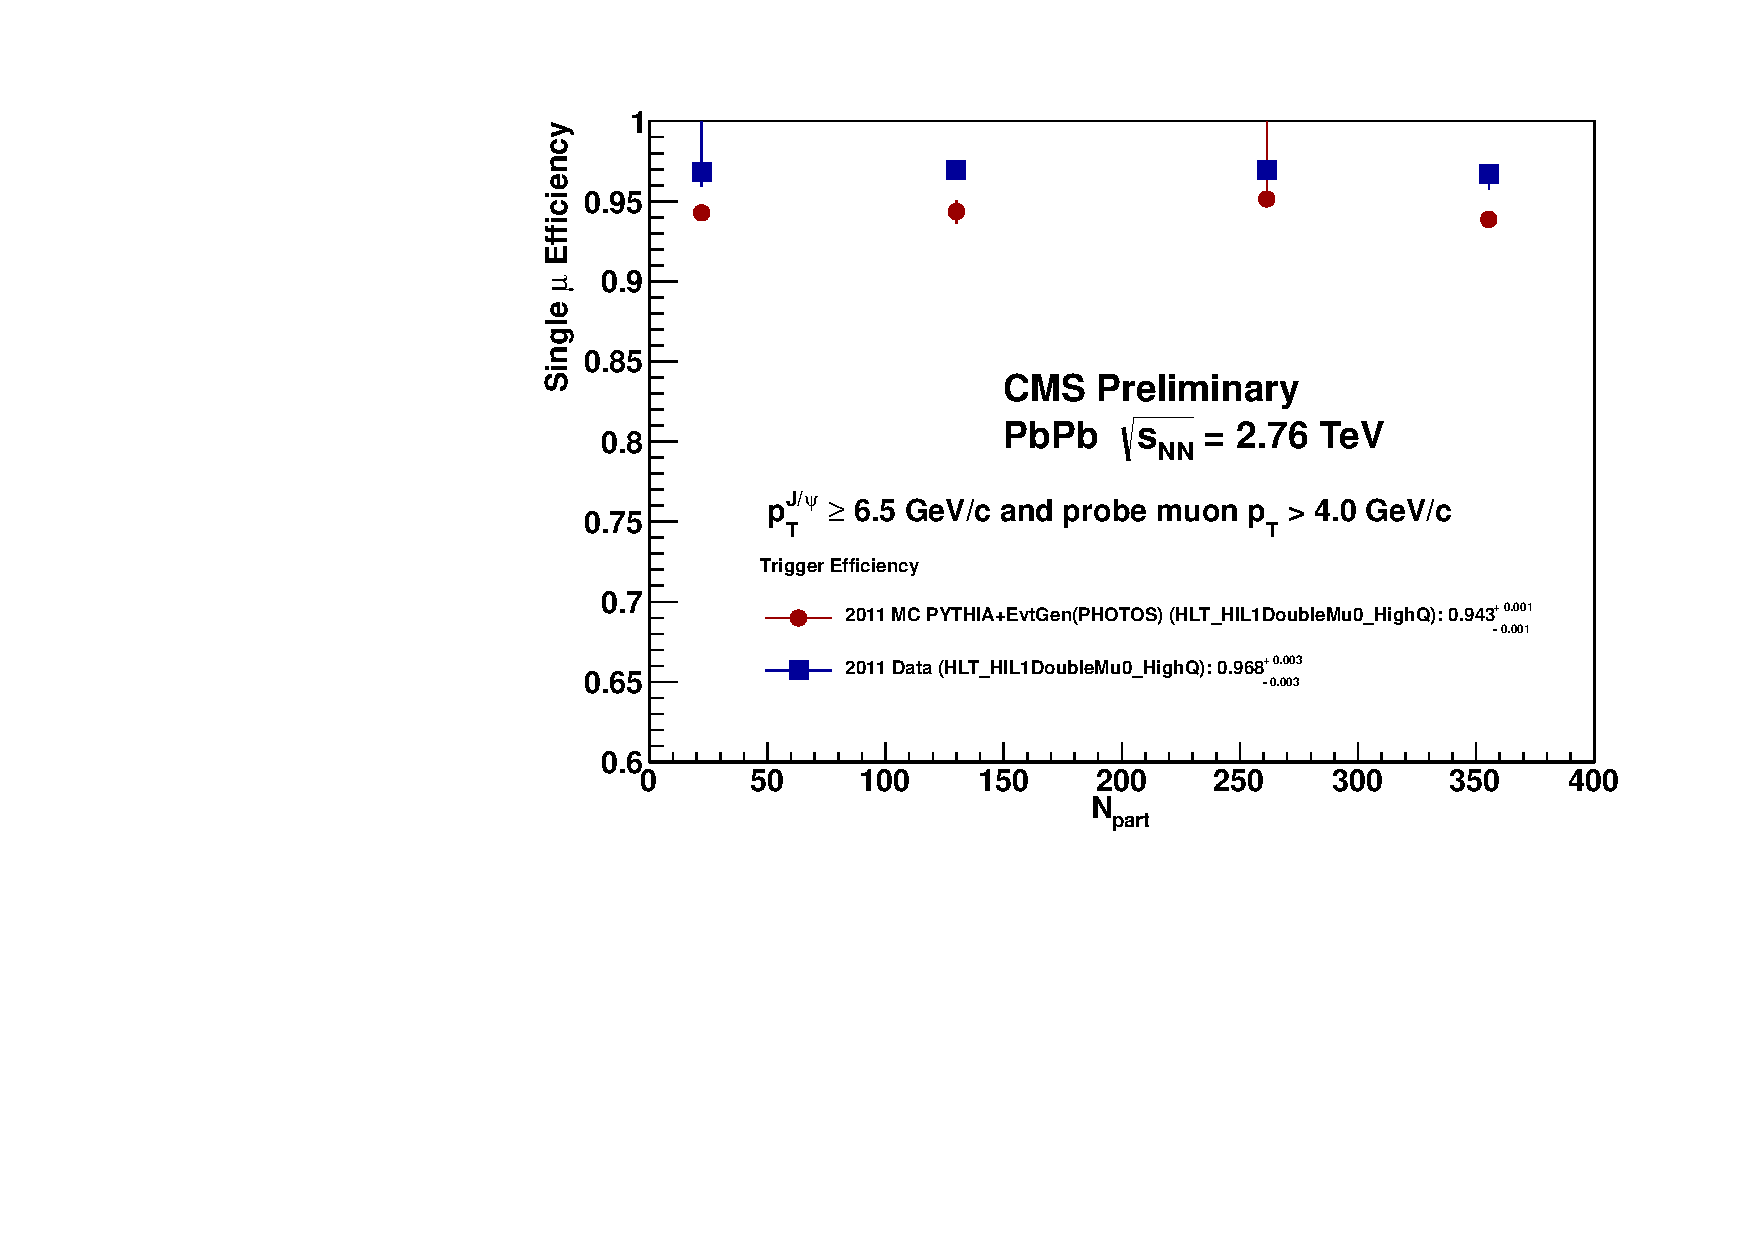
\includegraphics[width=0.6\textwidth]{figures/efficiency/Trg_Comp_HI_CNT_RD_MC_HighPt_notriggermatched}}
    \caption{Trigger efficiency measurements with tag and probe, and dependencies on probe muon \pt and pseudo-rapidity and event centrality. 
The efficiencies measured in the full samples are represented as open symbols and the corresponding numerical values are displayed for data and simulation. %TBD add MB/integrated point!
}
    \label{fig:tnpTrigEff}
  \end{center}
\end{figure}


%\subsubsection{Muon identification efficiency}

%In \fig{fig:tnpTrkFit} we show a good and a poor example of the fits to the passing and failing sample of tag and probe pairs for the muon identification efficiency measurement in data and MC, respectively. As noted above this includes the inner to outer track matching efficiency. Because standalone muons are used as probes, the momentum measured in the muon station has to be used in order not to have a different mass resolution in passing and failing probes (failing probes have no inner track matched, and thus no momentum measured with the inner tracker). This leads to a worse mass resolution than in the other two tag and probe pair mass distributions and a single Gaussian is used as signal pdf.

%Due to the poor momentum resolution also here we are subject to fluctuations and the \pt and $\eta$ dependence of the muon ID efficiency compares not so well between data and MC as shown in \fig{fig:tnpTrigEff}. The efficiency in data shows a \pt dependence not seen in MC, but it is unclear how significant this effect is due to the unknonw error on the MC. The agreement at high \pt is rather good. The tracking efficiency in data as function of $\eta$ is consistently lower than in MC. The \pt and $\eta$ integrated trigger efficiency is 89.2\,\% in MC and $78.8^{+8.8}_{-5.7}$\,\%. Half the difference is taken as a systematic uncertainty on the MC based efficiency correction. From the three efficiency comparisons between data and MC, this one has the largest systematic uncertainty. Adding all in quadrature gives a 6.7\,\% uncertainty on the single muon efficiency due to the data to MC comparison, which is a 13.4\,\% uncertainty on the \mumu pair efficiency.


\subsubsection{Muon identification efficiency}

%As for the trigger case, 
%Following the same idea as with the trigger efficiency 
We fit simultaneously the passing and failing tag-probe pairs mass distribution using a Crystal Ball function and (when needed to account for different resolutions) a Gaussian.
% to account for varying detector resolution. This time however a simple 
A first order polynomial is used to describe the background. For the MC case, a  Crystal Ball and an exponential describe the signal and background shapes. 

 T\&P mass fits for the muon identification efficiency are shown in \fig{fig:tnpMuIDFit}, for the integrated data and MC samples. 
These illustrate the considerably high level of background involved, in the heavy-ion environment. 
%The fits for all the centrality bins were well described with the previous choice of pdfs. 
%
Figure~\ref{fig:tnpMuIDEff} shows the muon identification efficiency measured as a function of probe \pt and pseudo-rapidity, and event centrality. 
A good agreement between data and simulation is observed. 
%The systematic is 0.4\%.
%we notice an improvement of the muon identification efficiency with respects to last year's results. This is due to the fact that this year we are using tracker muons as probes as opposed to \verb=hiGlobalPrimTrack=. Again no centrality dependency is observed.

\begin{figure}[hp]
  \begin{center}
    \subfigure[Data]{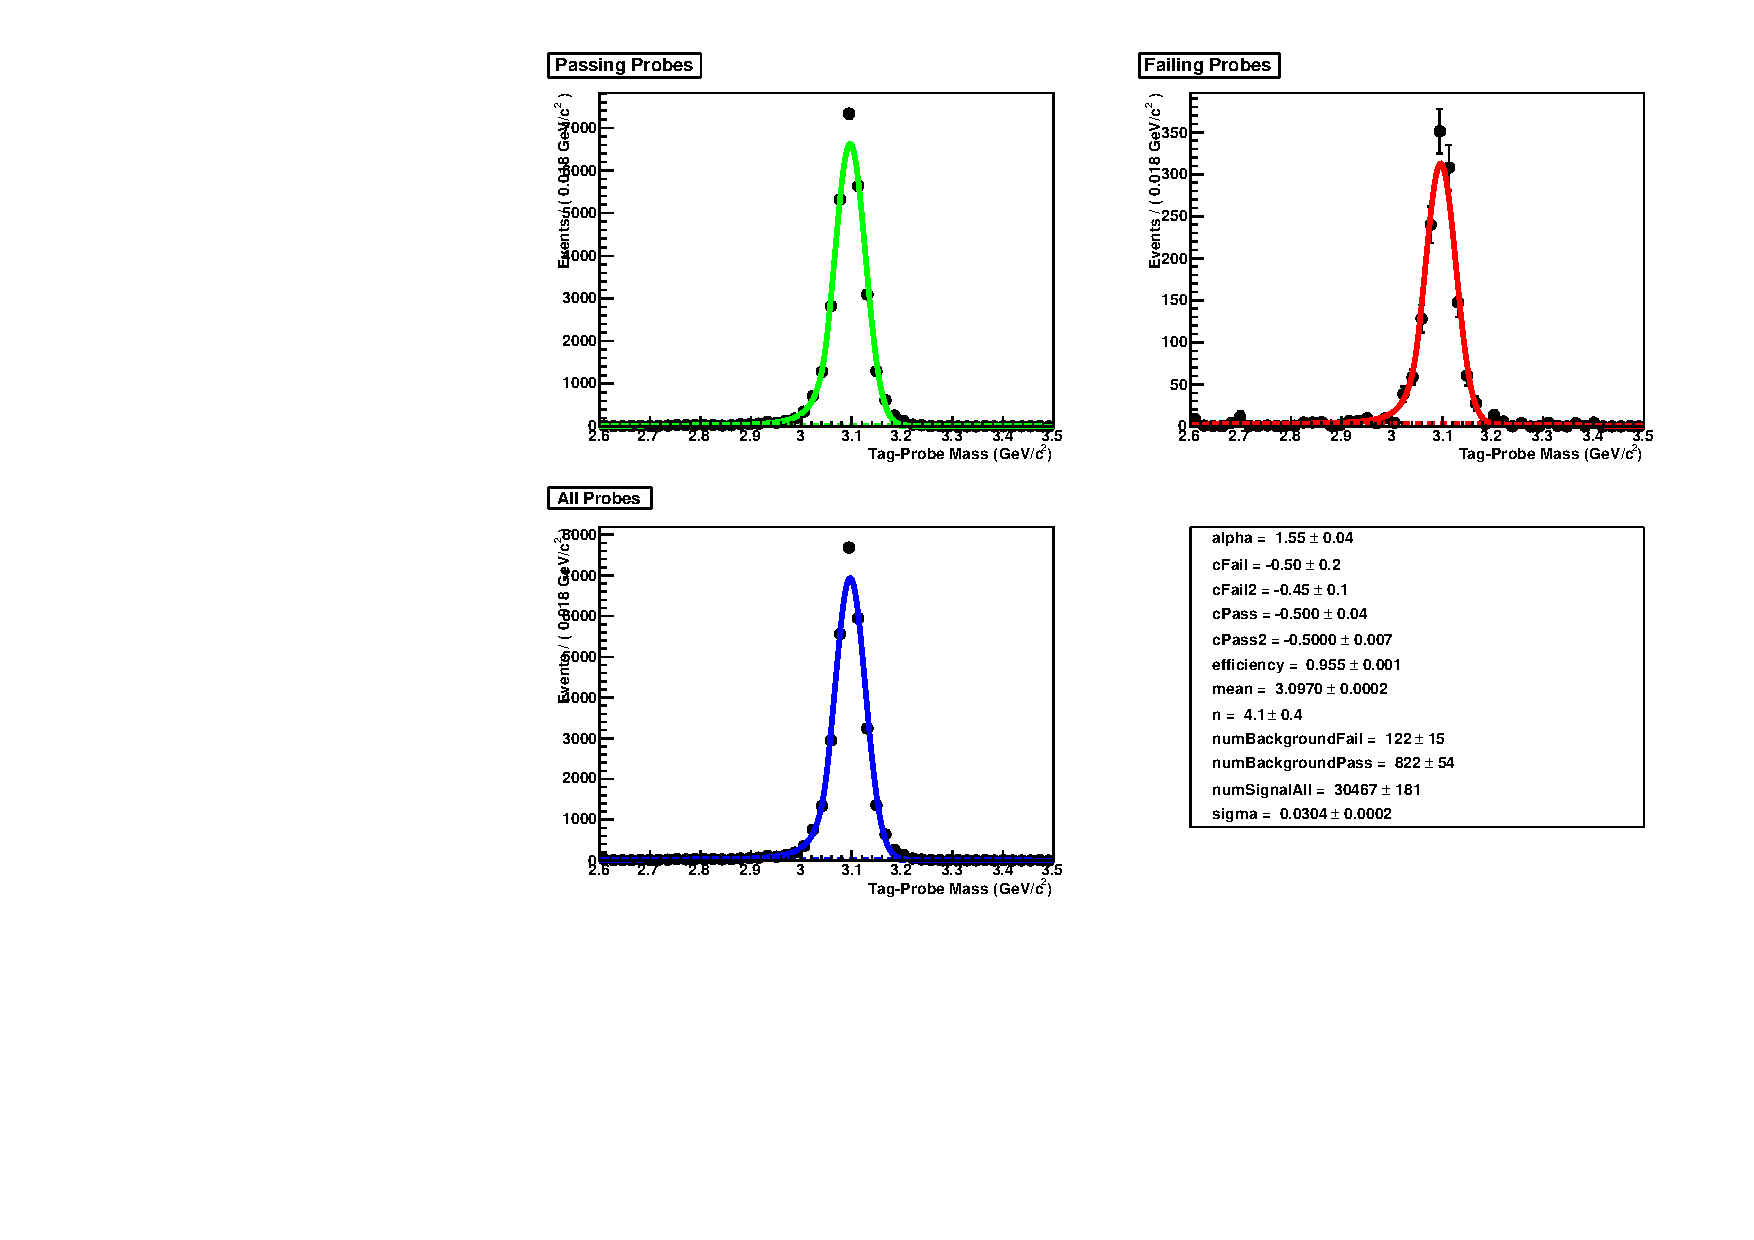
\includegraphics[width=0.9\textwidth]{figures/efficiency/MC_MuId_massfit_0100}}\hspace{1em}
    \subfigure[Simulation]{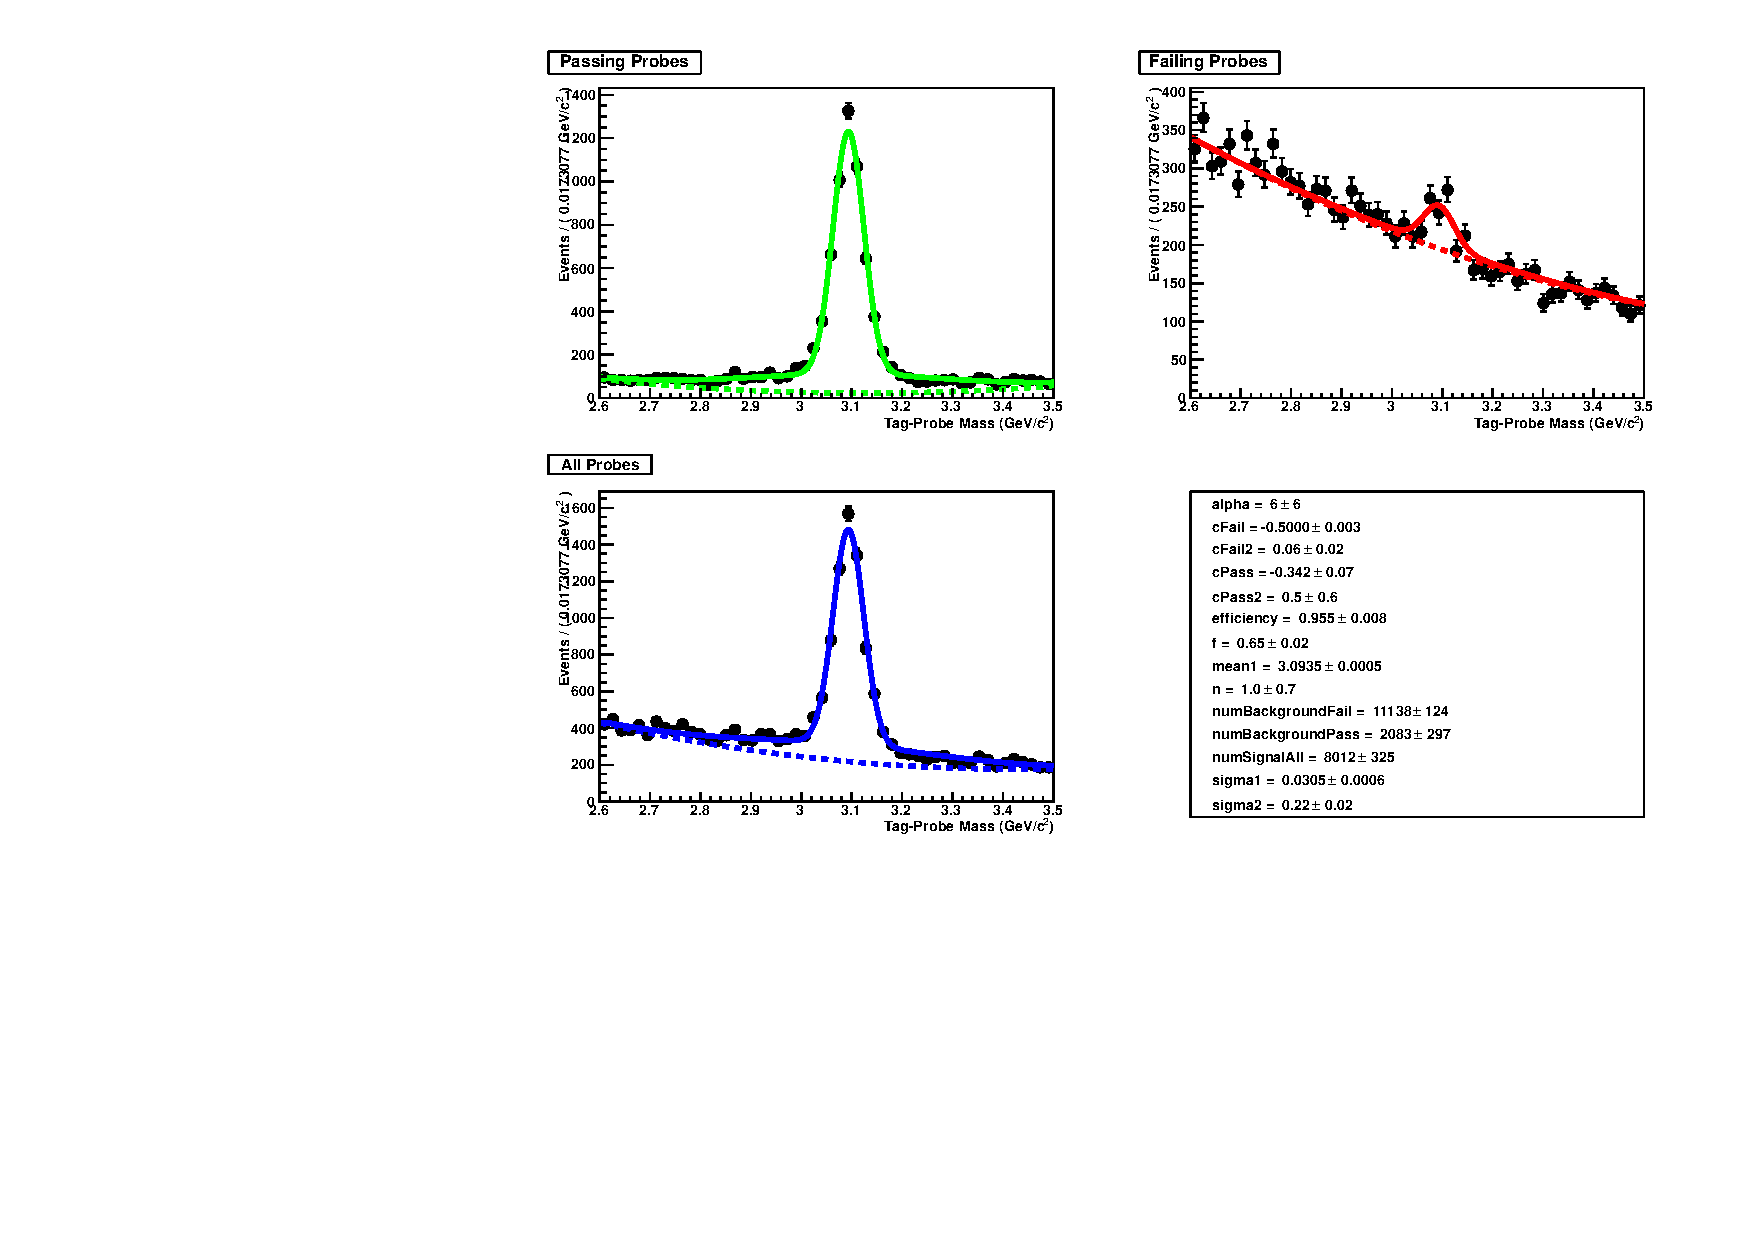
\includegraphics[width=0.9\textwidth]{figures/efficiency/RD_MuId_massfit_0100}}
    \caption{Examples of tag-probe pair mass fits for the muon identification efficiency in MC and data.}
    \label{fig:tnpMuIDFit}
  \end{center}
\end{figure}

\begin{figure}[hp]
  \begin{center}
    \subfigure[Muon id efficiency dependence on muon $\pt$.]{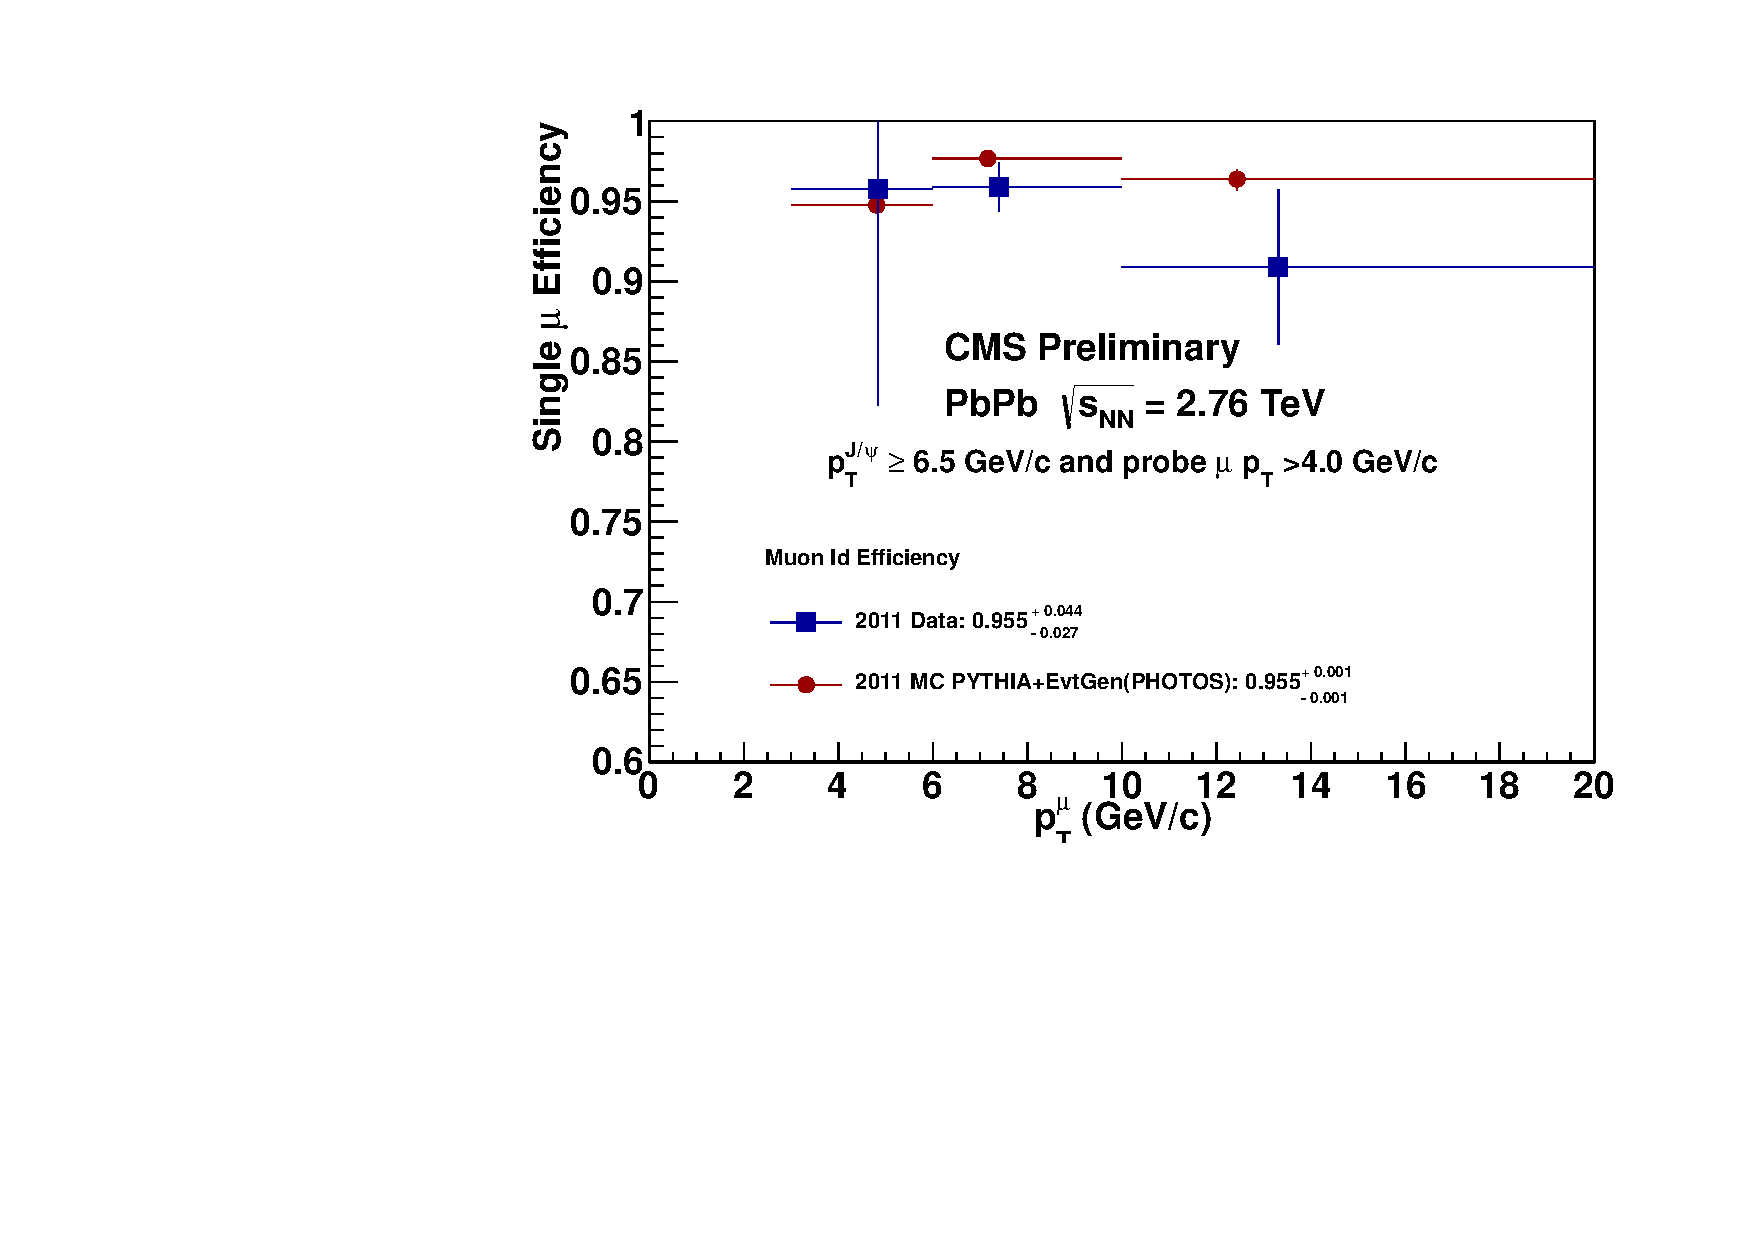
\includegraphics[width=0.6\textwidth]{figures/efficiency/MuID_Comp_pt}} \\ %\hspace{1em}
    \subfigure[Muon id efficiency dependence on muon $\eta$.]{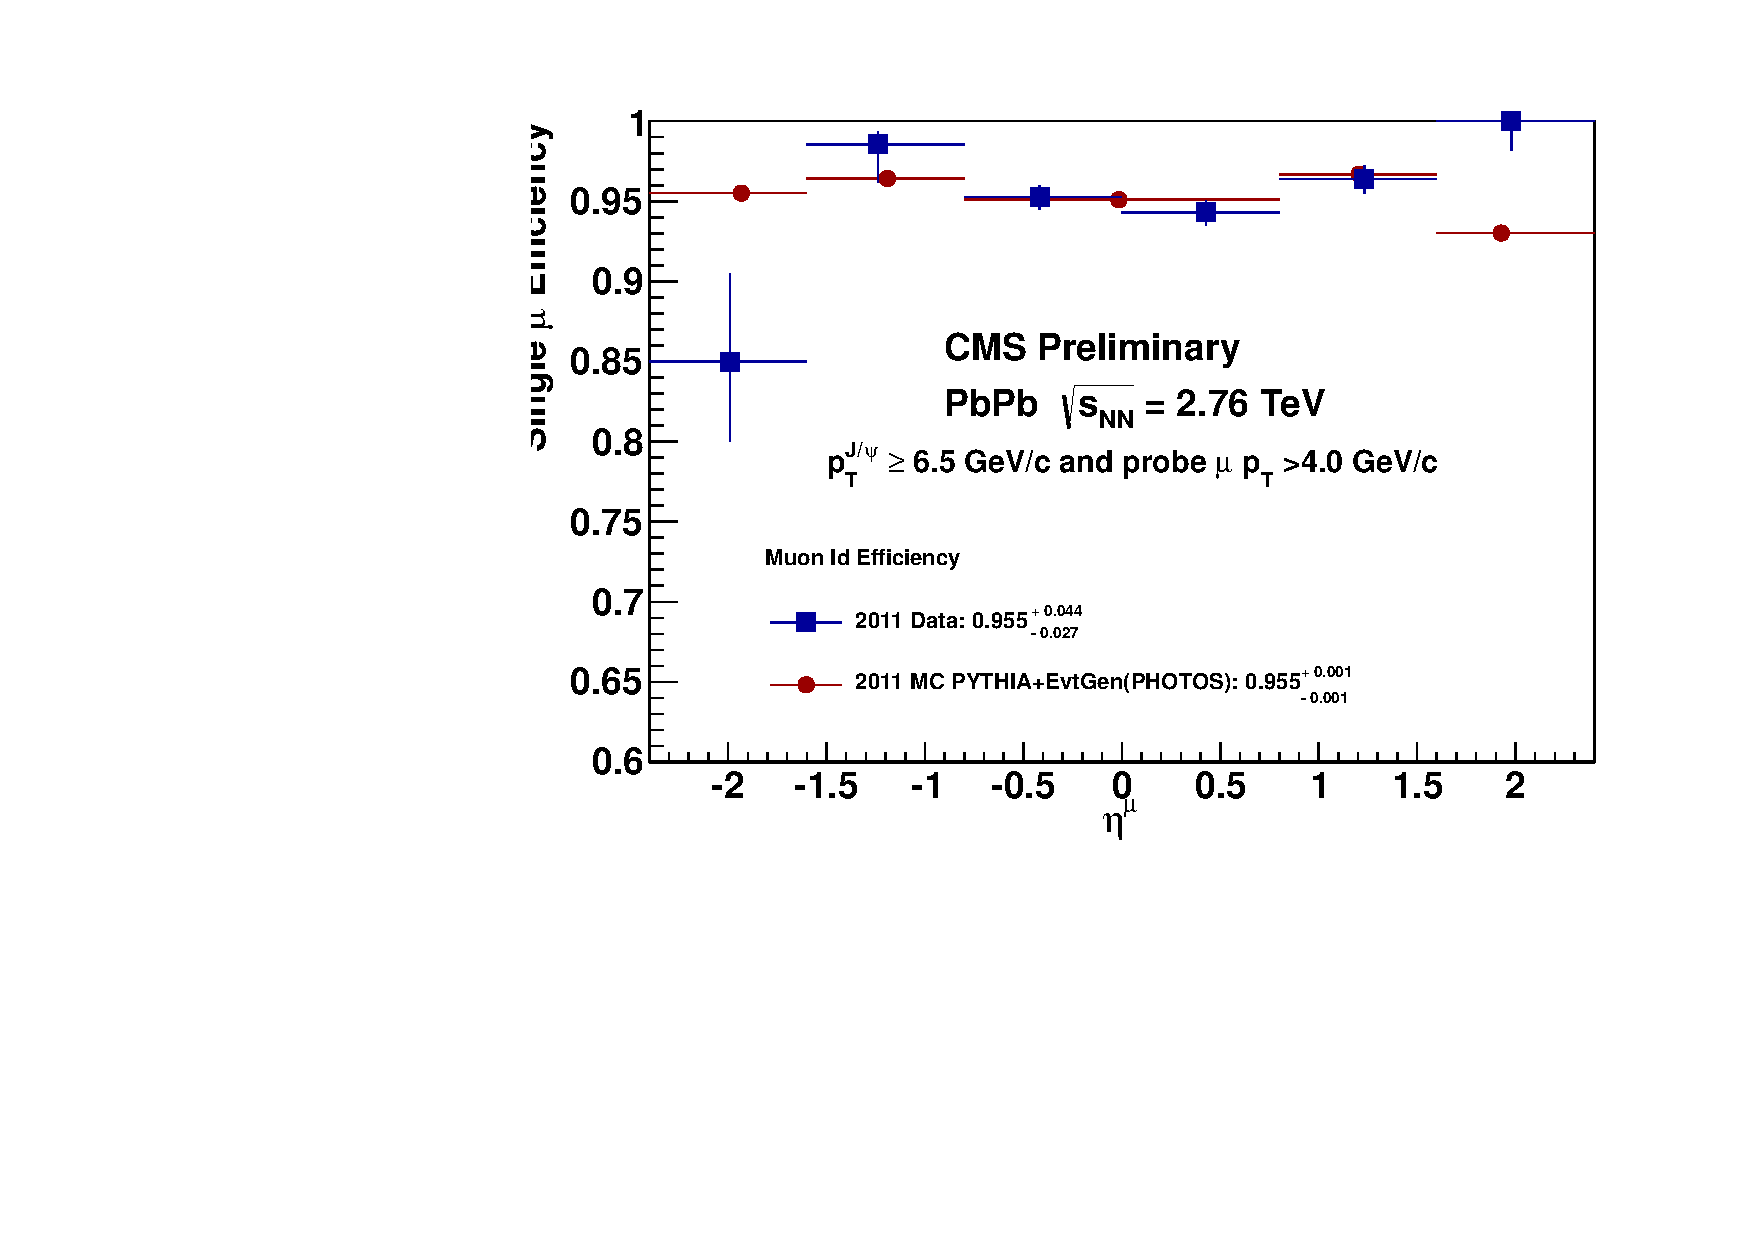
\includegraphics[width=0.6\textwidth]{figures/efficiency/MuID_Comp_eta}} \\
    \subfigure[Muon id efficiency dependence on event centrality.]{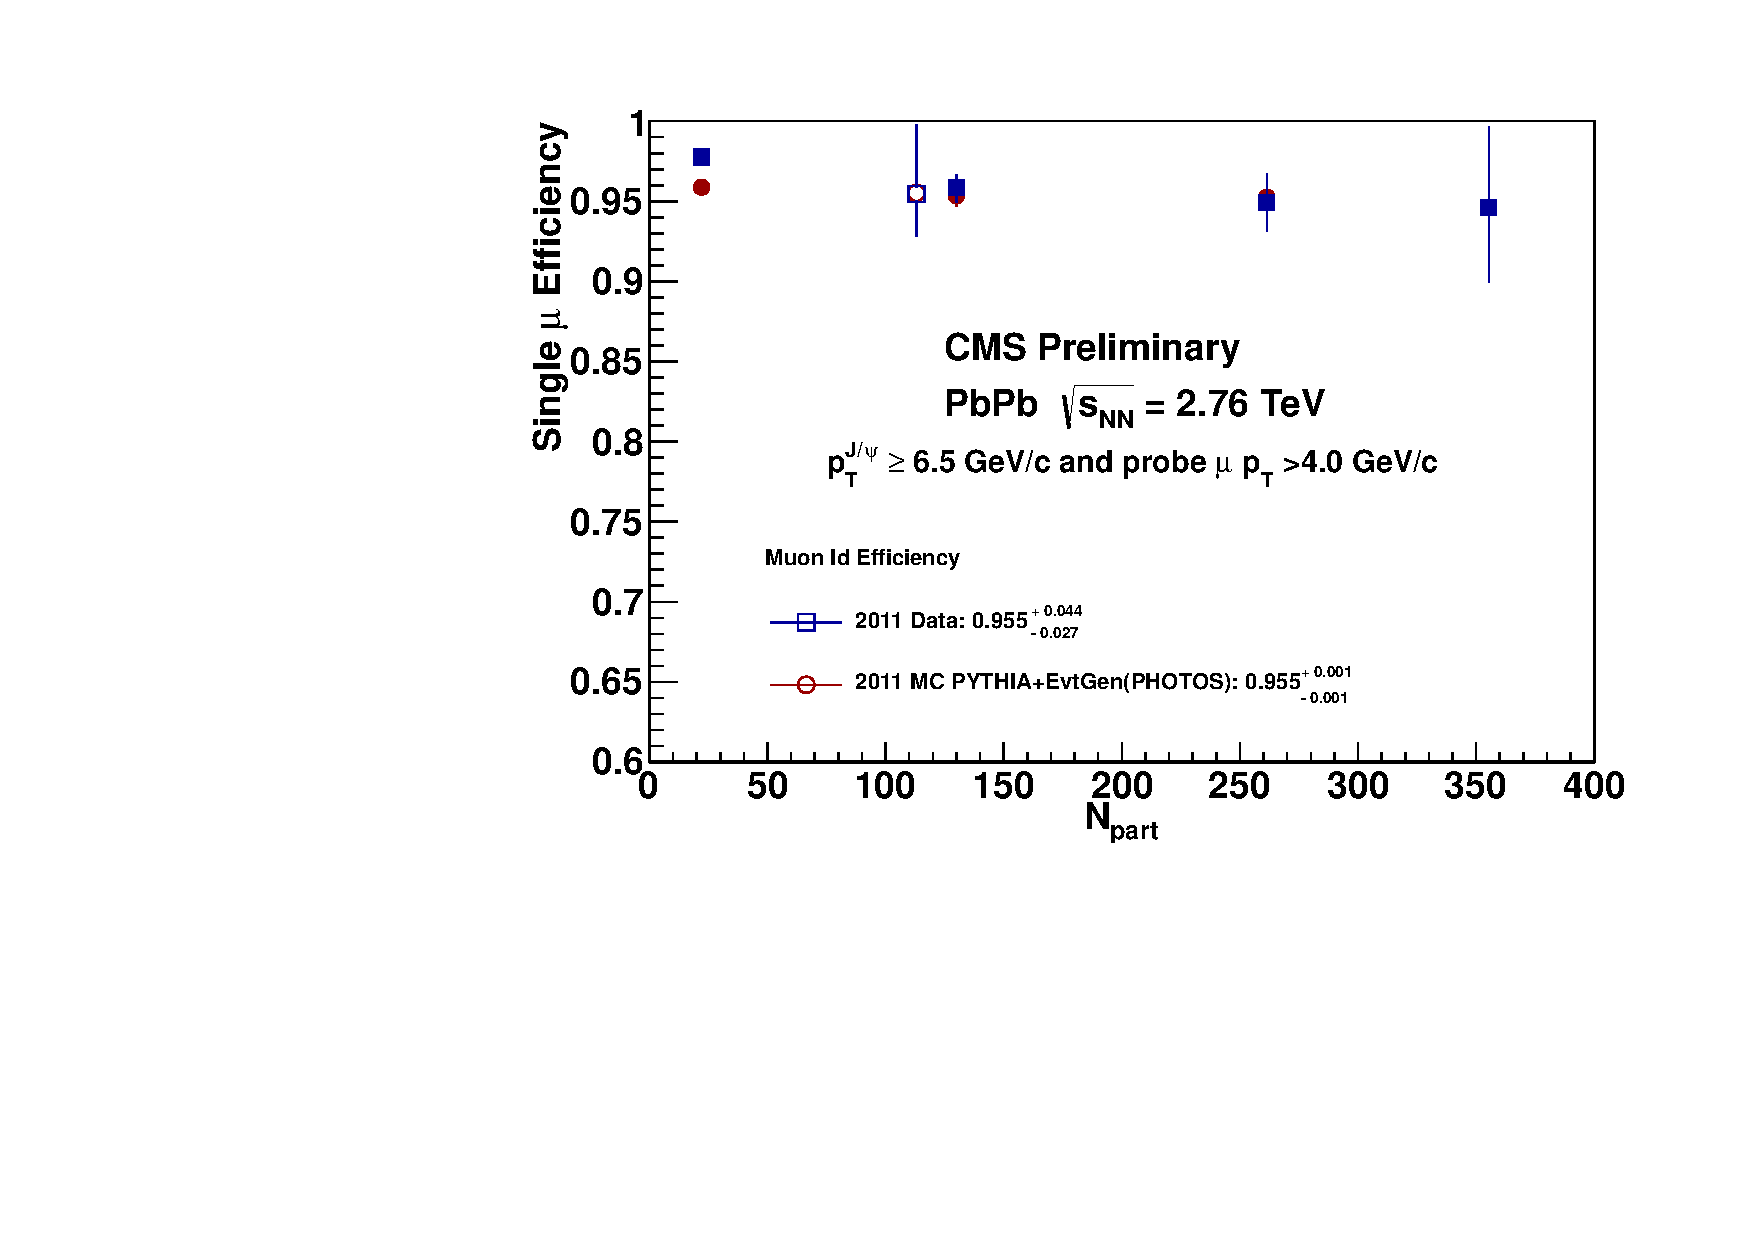
\includegraphics[width=0.6\textwidth]{figures/efficiency/MuID_Comp_cent}}
    \caption{Muon identification efficiency measurements with tag and probe, and dependencies on probe muon \pt and pseudo-rapidity and event centrality. The efficiencies measured in the full samples are represented as open symbols and the corresponding numerical values are displayed for data and simulation.}
%Comparison of the trigger efficiency measured with Tag and Probe in 2011 \emph{(blue squares and pink stars)} and 2010  \emph{(red circles and green triangles)} data, as function of \pt \emph{(left)}, $\eta$ \emph{(right)} and centrality \emph{(bottom)}.}
    \label{fig:tnpMuIDEff} %TBD: update these
  \end{center}
\end{figure}


\subsubsection{Tracking efficiency}

%Given the poorer mass resolution (based on stadalone muon \pt probe measurements), an enlarged fitting range is used. 
%In addition to the \Jpsi, also the contribution from the $\Psi^\prime$ needs to be accounted for in the mass fits.

The fits for the tracking efficiency are challenging due to the poor resolution of the standalone muons used as probes. For the same reason, an enlarged fitting range is used. 
A Crystal Ball (and an additional Gaussian when needed to account for different event resolutions, eg for the MC fits) is chosen to describe the signal shape with all its parameters left to float. The background is described by a third order polynomial. 
%Notice that the invariant mass region used was considerably greater. For the MC case we used a Crystal Ball plus a Gaussian in order to account for varying detector resolution effects. 
%However, it must be noticed that the final efficiencies presented here were not extracted from the fitting results but from a counting method which is, together with fitting and side band subtraction, another option in the T\&P package. 

T\&P mass fits for the tracking case are shown in \fig{fig:tnpTrkFit}, for the integrated data and MC samples.
These illustrate the considerably large level of background involved, and the degraded mass resolution. 
%No dimuon-muon \pt selection is applied as the stadalone muon measurement is not sufficiently precise.  
%
Shown in \fig{fig:tnpTrkEff} is the tracking efficiency as function of the probe muon \pt and rapidity and event centrality. % for all \Jpsi. 
The MC is seen to overestimate the data, by about 5\%.
%MC and data  show a very good agreement, respectively with 85.0\% and 83.7$^{0.57}_{0.53}$\% for single muon efficiency. 
%Twice this difference, 4.6\%, is used as a  systematics on the corrected dimon yields. 
%No significant centrality dependence is observed in MC, while in data, there seem to be a drop of the efficiency going to the peripheral collisions. 
%This goes in the opposite direction than expectations that efficiency would get lower in a very dense environment but is probably just illustrating fake efficiency in the central bins.
%
%We note this particular measurement is challenging, as anticipated. The measured efficiency values appear to be relatively higher than expected. The systematic is 10.5\%.
%We have tried to switch to tracker muons as probes but it didn't help much as the background is fluctuating a lot with STA resolution. %??? tracker muon contain tracker info, so these are not unbiased probles, right?
%In conclusion,  T\&P tracking results are still being studied. 
%Further studies are still being pursued, including of stricter tag/probe selection, to attempt to better understand the background shape. 
%Some cuts on the tags \pt might help understand the background shape better.

\begin{figure}[hp]
  \begin{center}
    \subfigure[Data]
    {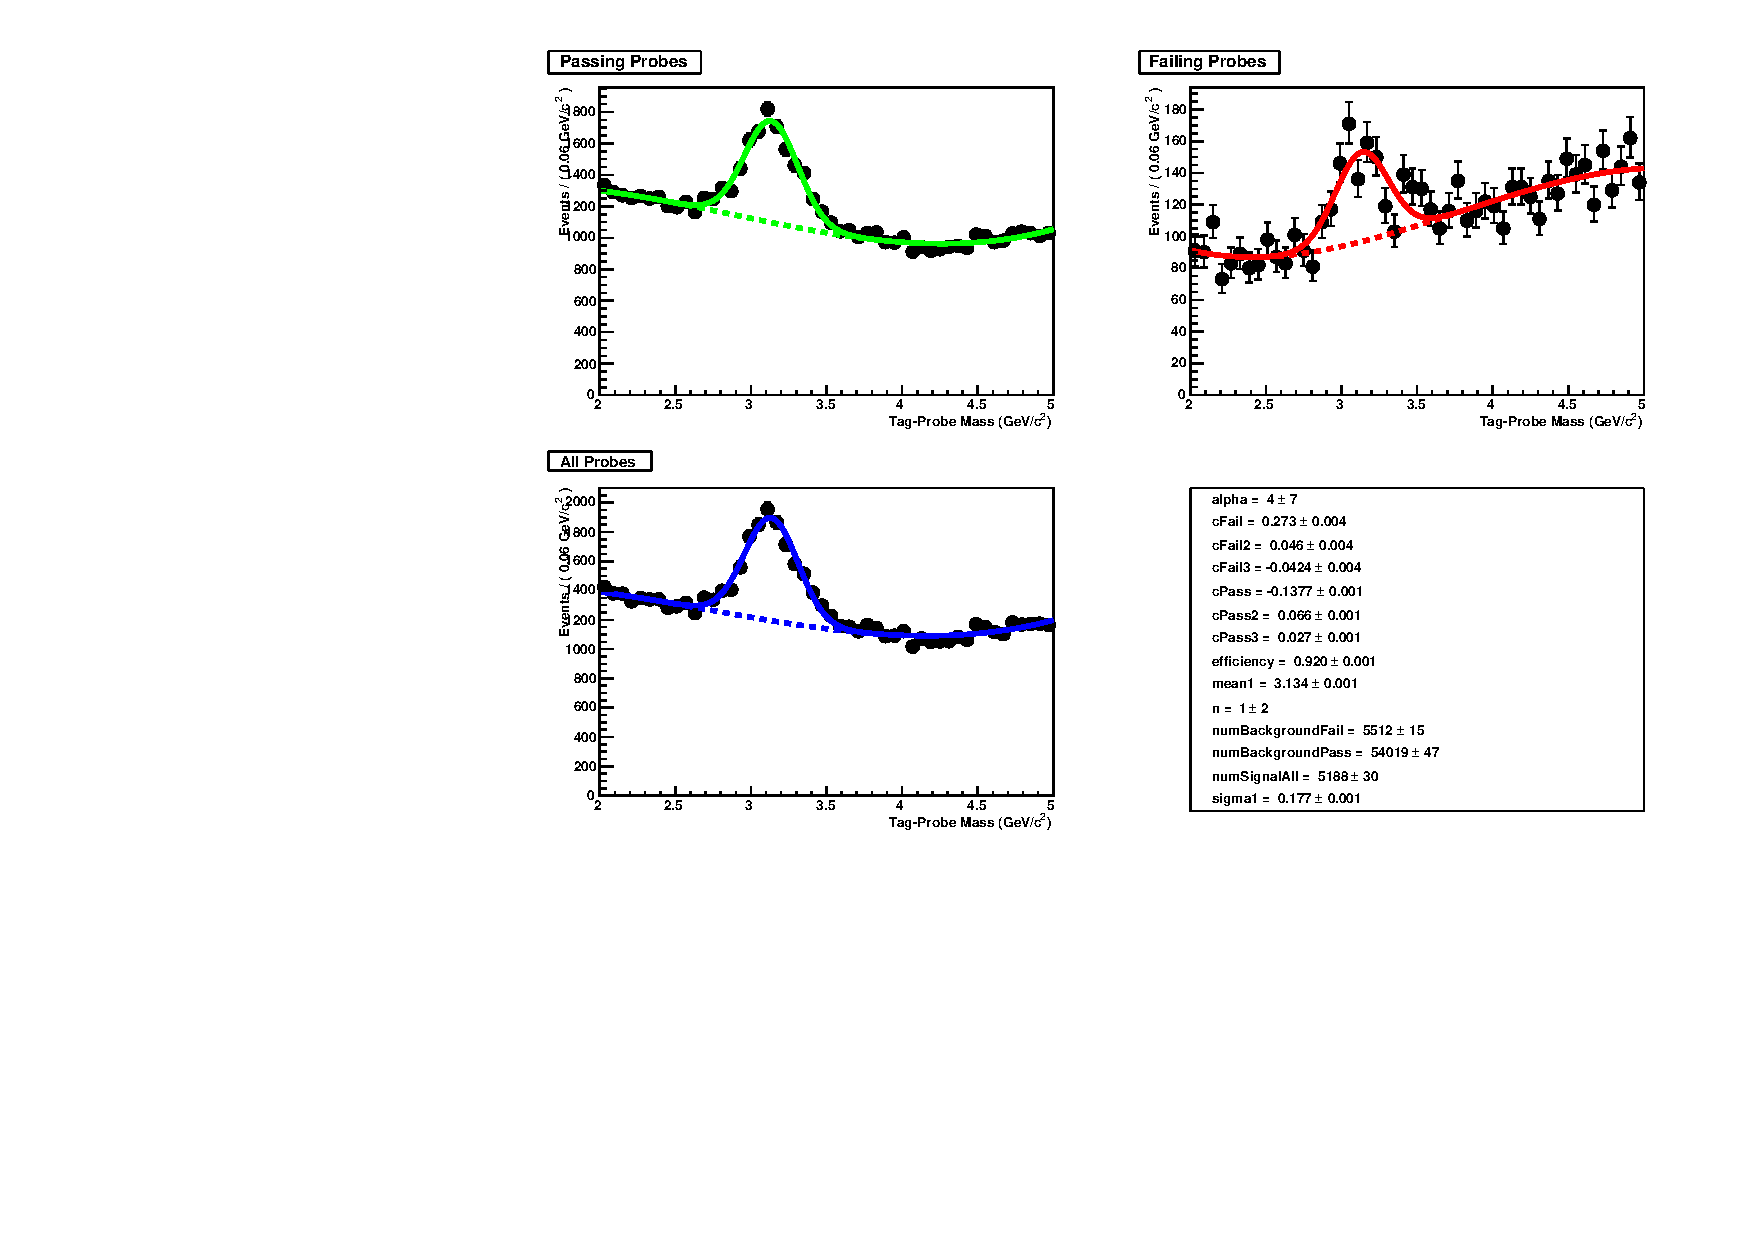
\includegraphics[width=0.9\textwidth]{figures/efficiency/RD_Trk_massfit_0100}}\hspace{1em}
    \subfigure[Simulation]
    {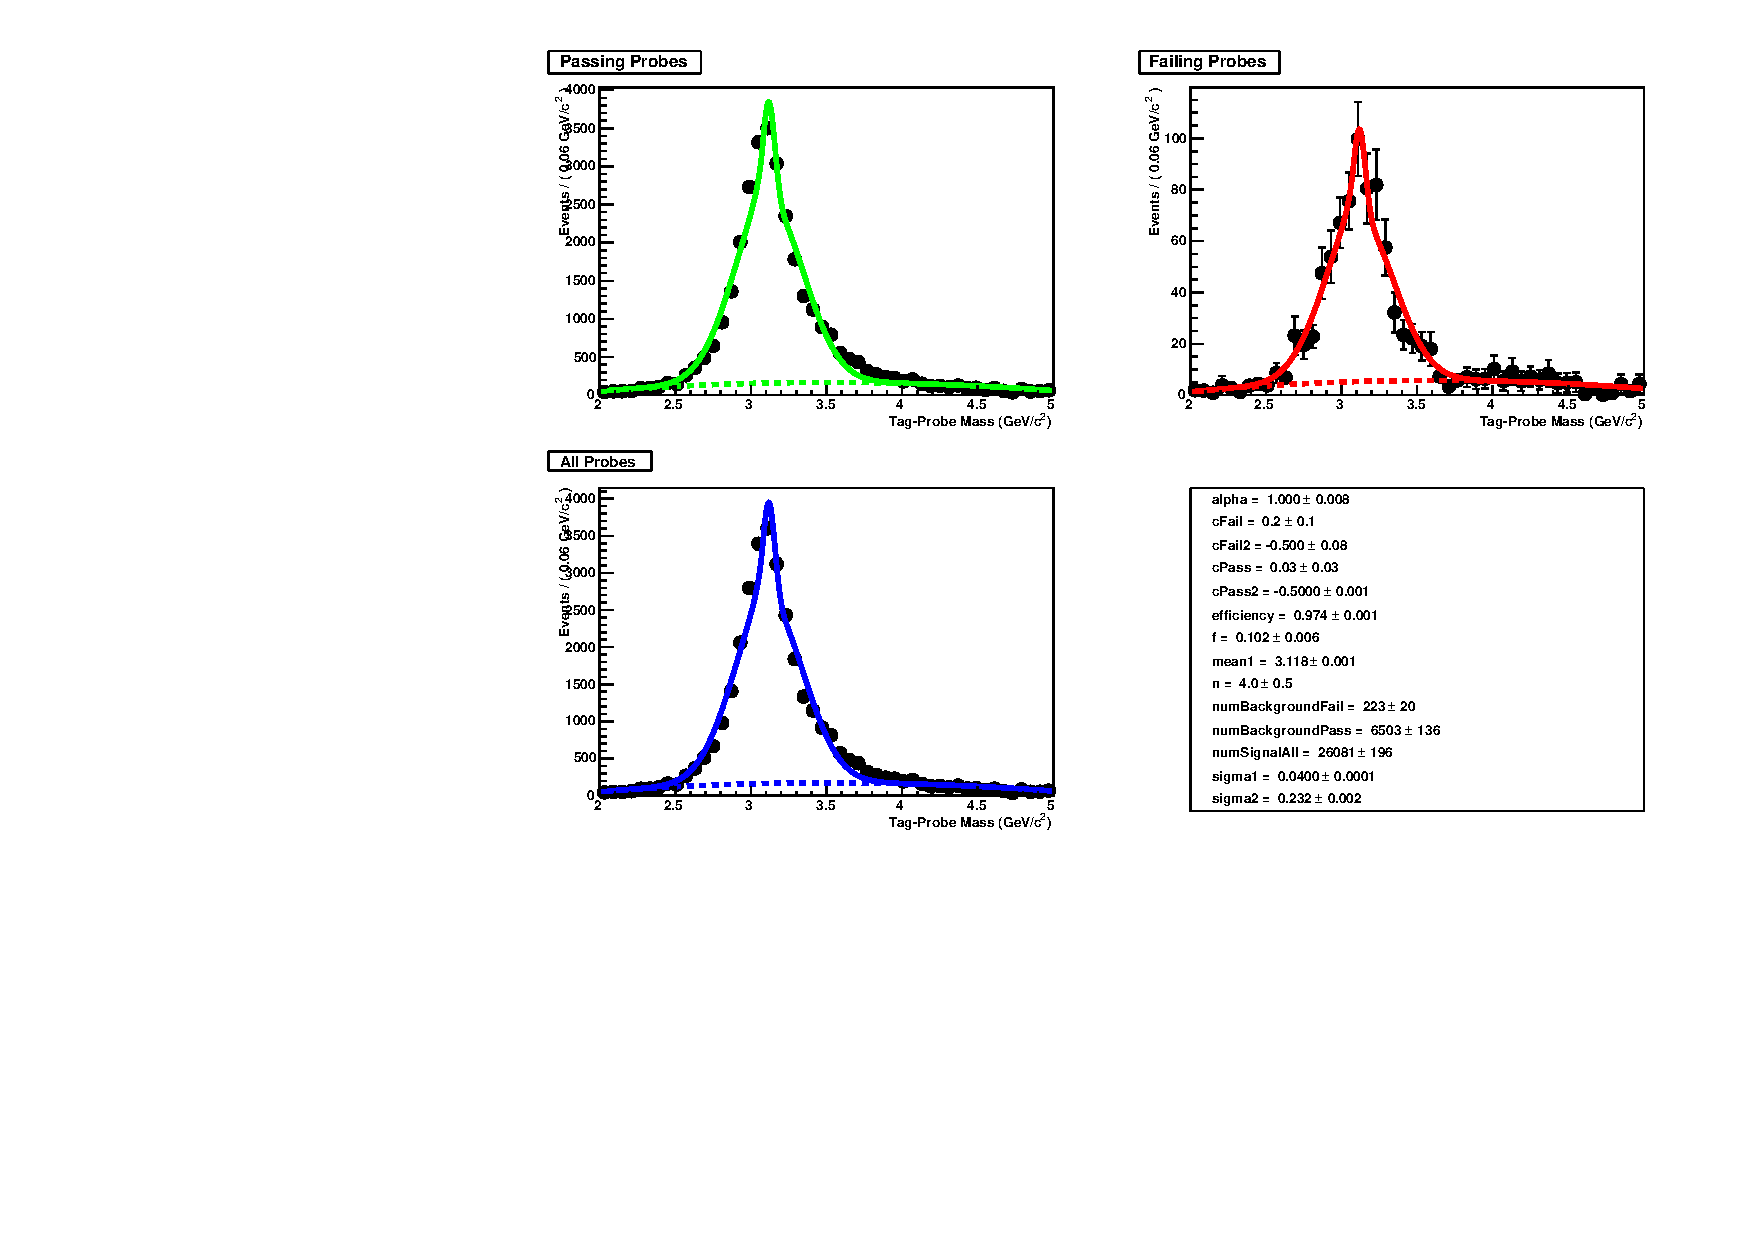
\includegraphics[width=0.9\textwidth]{figures/efficiency/MC_Trk_massfit_0100}}
    \caption{Examples of tag-probe pair mass fits for the inner tracking efficiency.}
    \label{fig:tnpTrkFit}
  \end{center}
\end{figure}

\begin{figure}[hp]
  \begin{center}
    \subfigure[Tracking efficiency dependence on muon $\pt$.]{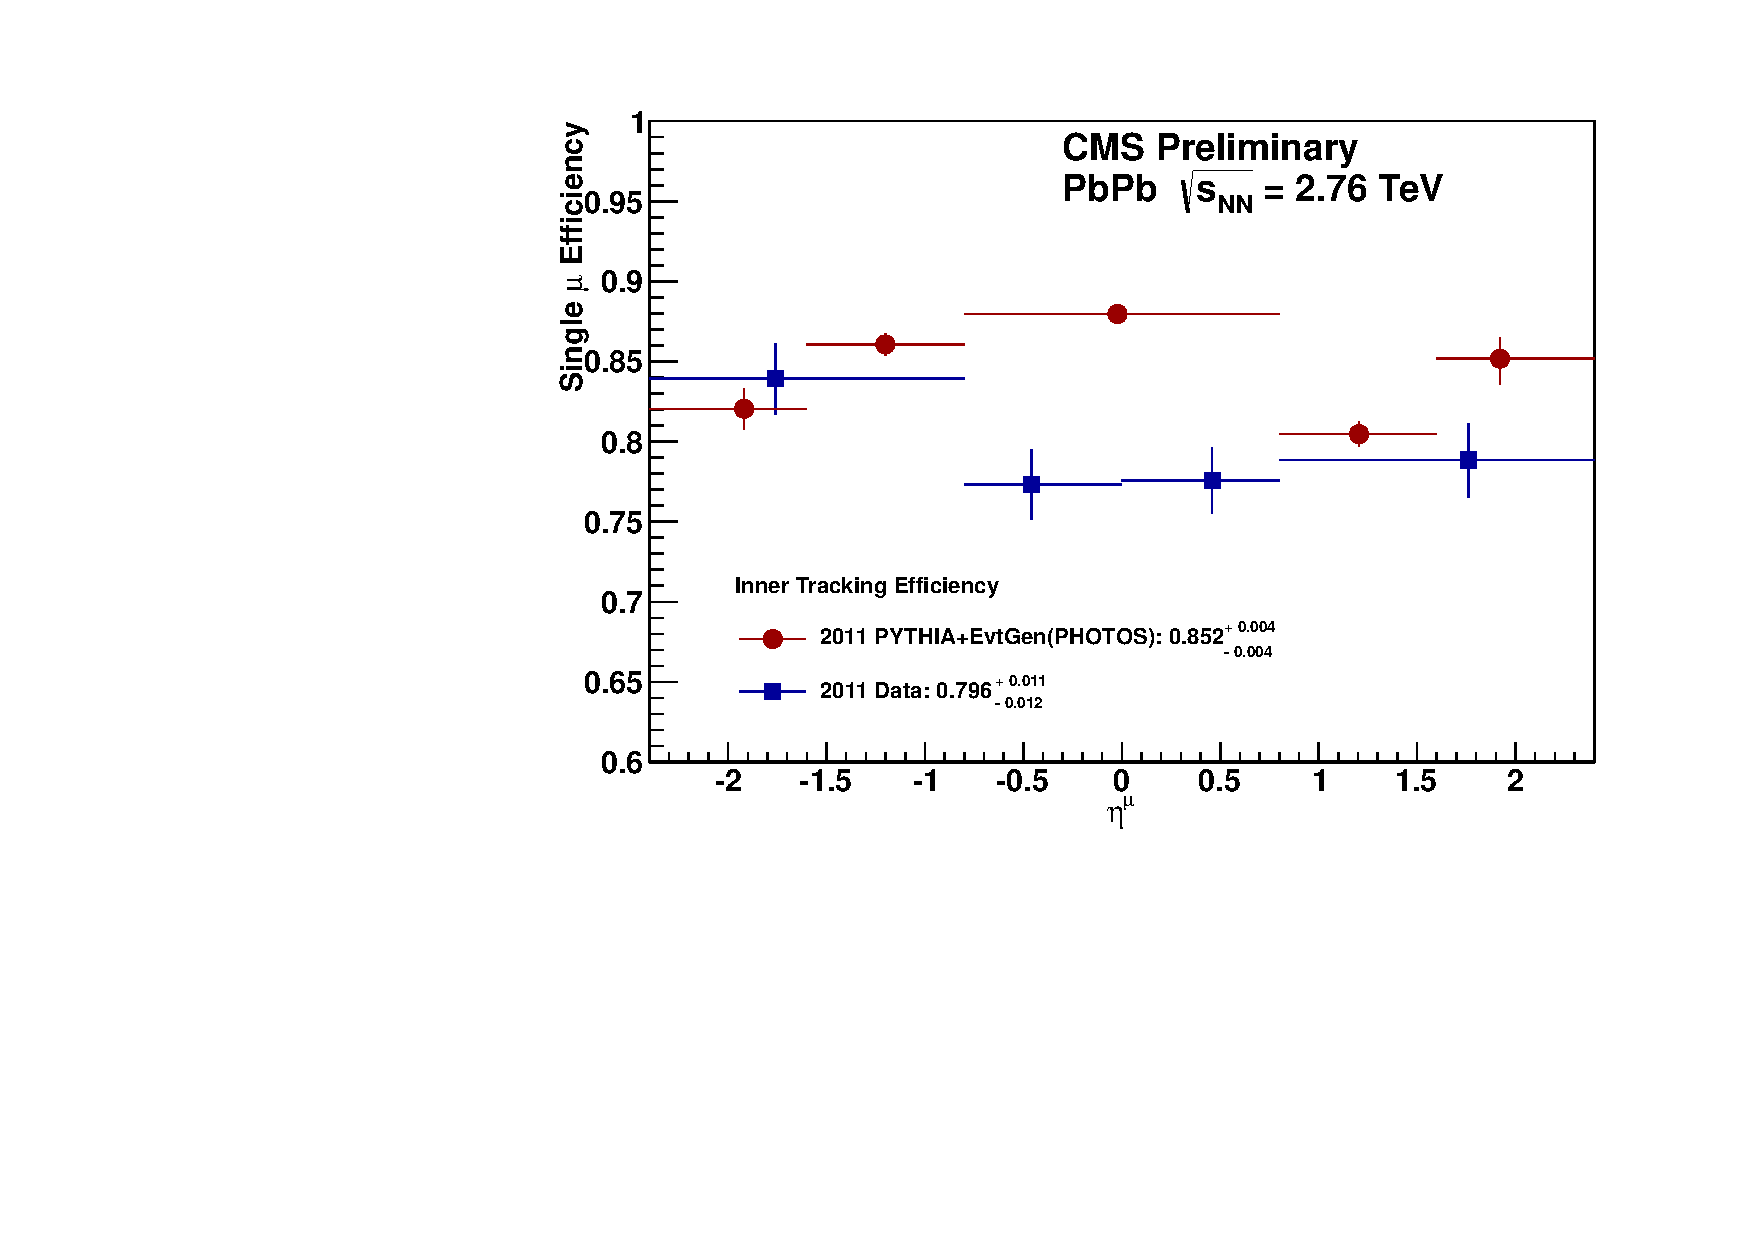
\includegraphics[width=0.6\textwidth]{figures/efficiency/Trk_Comp_eta_MC_RD_highPt_notriggermatched}}  \\ %\hspace{1em}
    \subfigure[Tracking efficiency dependence on muon $\eta$.]{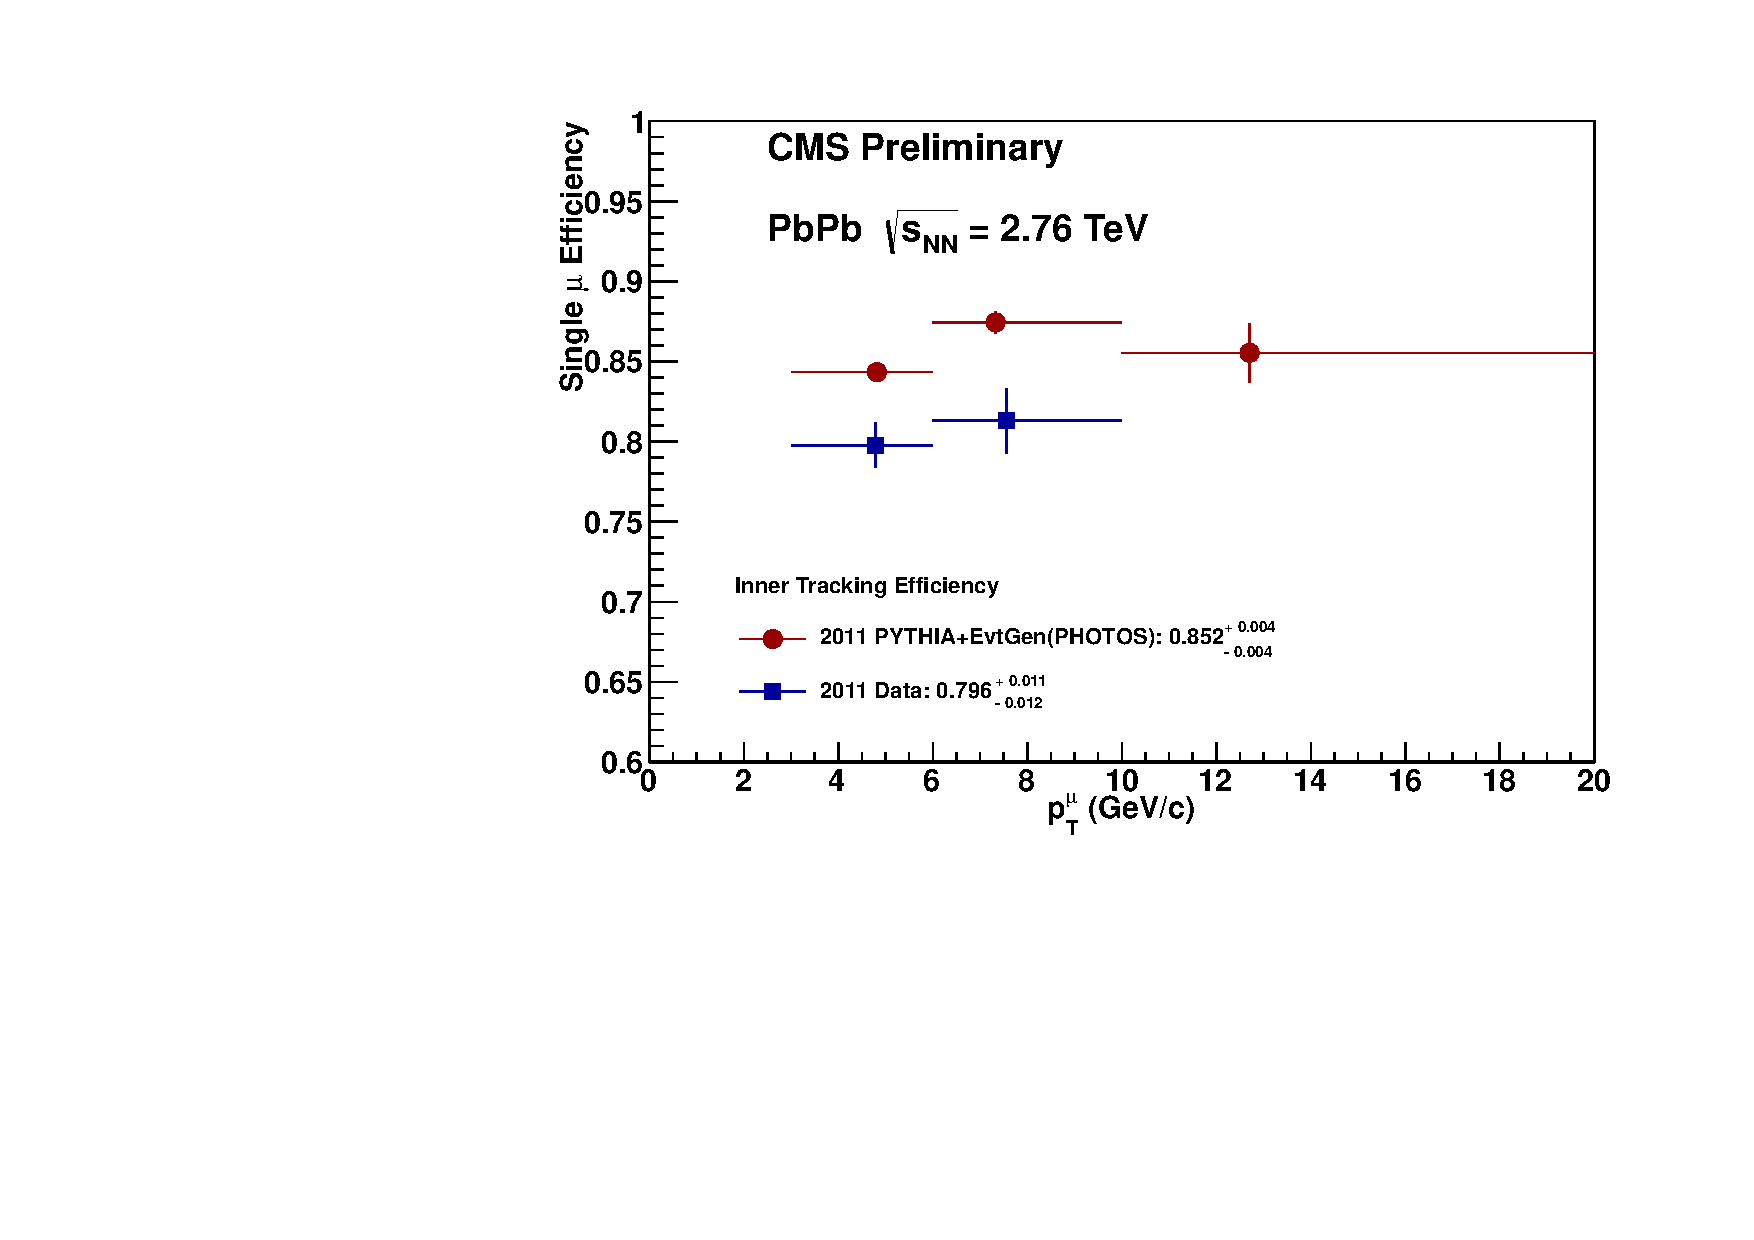
\includegraphics[width=0.6\textwidth]{figures/efficiency/Trk_Comp_pt_MC_RD_HighPt_notriggermatched.pdf}} \\
    \subfigure[Tracking efficiency dependence on event centrality.]{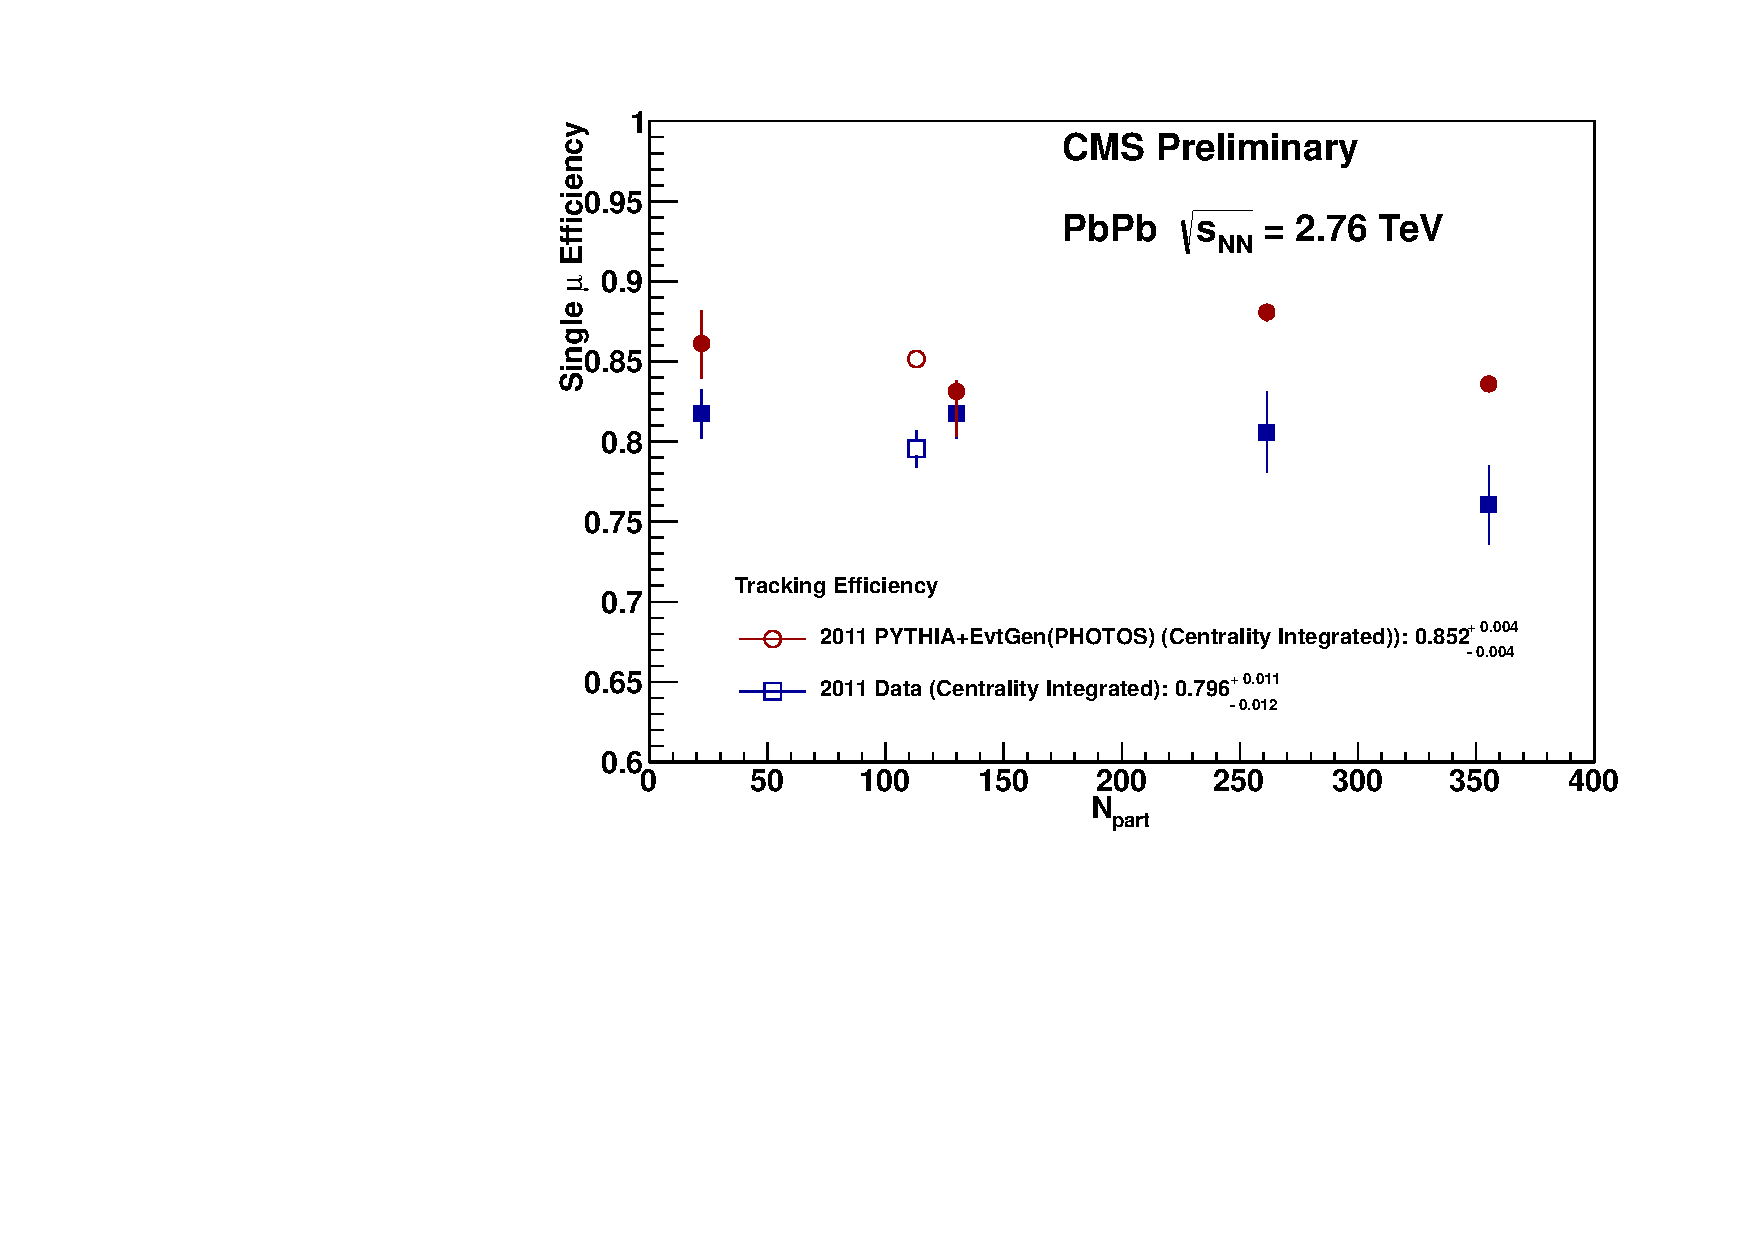
\includegraphics[width=0.6\textwidth]{figures/efficiency/Trk_Comp_CNT_MC_RD_highPt_notriggermatched}}
    \caption{Tracking efficiency measurements with tag and probe, and dependencies on probe muon \pt and pseudo-rapidity and event centrality. The efficiencies measured in the full samples are represented as open symbols and the corresponding numerical values are displayed for data and simulation.}
    \label{fig:tnpTrkEff} %TBD: update!
  \end{center}
\end{figure}

Finally we summarize in Table~\ref{tab:TnPEffTable} all the efficiency estimations as a function of centrality, based on the full data and simulation \PbPb samples.
%
\begin{table}[h!]
\begin{center}
\caption{Tag and probe efficiency measurements in \PbPb data and simulation; 
an acceptance cut $\pt^{\mu} > 4.0 \GeVc$ on the probe muons is applied; 
values are in percent, and errors are statistical only.} 
%n and reconstruction efficiency for data and MC. .
\label{tab:TnPEffTable}
\begin{tabular}{c|cc|cc|cc}
\hline
          \PbPb & \multicolumn{2}{c}{Muon Identification} & \multicolumn{2}{|c}{Trigger} & \multicolumn{2}{|c}{Tracking} \\
centrality& MC   & data & MC   & data & MC   &data   \\
\hline
0-10\%    & $94.6 \pm 0.2$ & $94.6 \pm 5.0$ & $93.9 \pm 2.1$ & $96.7 \pm 0.5$ & $83.6 \pm 0.4 $ & $76.1 \pm 2.5 $   \\
10-20\%   & $95.3 \pm 0.3$& $94.9 \pm 1.8$& $95.1 \pm 4.8$ & $96.9 \pm 0.5$ & $88.0 \pm 0.6 $ & $80.6 \pm 2.5 $  \\
20-50\%   & $95.3 \pm 0.2$ & $95.8 \pm 2.5$ & $94.4 \pm 0.7$ & $96.7 \pm 0.4$& $ 83.1 \pm 2.0 $ & $81.7 \pm 1.5 $ \\
50-100\%  & $95.9 \pm 0.6$ & $97.8 \pm 0.8$ & $94.3 \pm 0.7$ & $96.8 \pm 3.2$& $86.1 \pm 2.0 $ & $81.7 \pm 1.5 $  \\
0-100\%   & $95.5 \pm 0.1$ & $95.5 \pm 4.4$ & $94.3 \pm 0.1$ & $96.8 \pm 0.2$ & $85.2 \pm 0.3$ & $79.6 \pm 1.2$  \\

%\begin{tabular}{c|c|c}

%  \hline
% & data & MC \\
%  \hline
%  Trigger              &  $ 97.2 \pm  0.3 $ & $ 94.3 \pm 0.1 $ \\
%  Muon Identification  &  $ 95.5 \pm  0.8 $ & $ 95.5 \pm 0.1 $ \\
%  Tracking             &  $ 85.2 \pm  0.3 $ & $ 79.6 \pm 1.2 $ \\
\hline
\end{tabular}
\end{center}
\end{table}


Table~\ref{tab:TnPEffTablepp} also summarizes the tag and probe results obtained from the \pp data and MC datasets. These studies were performed in the analysis documented in Ref.~\cite{CMS_PAS_HIN-10-006}. While different selection criteria were employed therein, which prevents a direct comparison of results for \pp and \PbPb, this may be used for the purpose of data--simulation systematic estimation.


\begin{table}[h!]
\begin{center}
\caption{Tag and probe efficiency measurements in \pp data and simulation; 
an acceptance cut $\pt^{\mu} > 4.0 \GeVc$ on the probe muons is applied; 
values are in percent, and errors are statistical only; results from~\cite{CMS_PAS_HIN-10-006}.} 
\label{tab:TnPEffTablepp}
\begin{tabular}{c|cc|cc}
\hline
& \multicolumn{2}{|c}{Trigger} & \multicolumn{2}{|c}{Tracking} \\
& MC   & data & MC   &data   \\
\hline
\pp &
​0.943 $\pm$ 0.002 & 0.925 $\pm$ 0.006 &
​0.846 $\pm$ 0.010 &​0.82  $\pm$ 0.02 \\
\hline
\end{tabular}
\end{center}
\end{table}

\end{chapter}
